% \chapter{Bridge Bearings}
\chapter{桥梁支座}\label{chp:bridge-bearings}
% \section{Introduction}
\section{简介}
% Bearings are a critical element within overall bridge systems. Although they represent only a small part of the overall structure cost, they can potentially cause significant problems if they don’t function properly or if possible maintenance, retrofit, or replacement strategies are not envisioned and well planned at the design stage. Bridge superstructures experience translational movements and end rotations caused by traffic loading, thermal effects, creep and shrinkage, wind and seismic forces, initial construction tolerances, and other factors. Bridge bearings are designed and built to accommodate these movements and rotations while supporting required gravity loads, transmitting those loads to the substructure, and providing necessary restraint for the superstructure. Proper functioning of bridge bearings is assumed in the analysis and design of overall bridge systems. Bearing failure or improper behavior can lead to significant changes in load distribution and overall structural behavior that are not accounted for in the design, and can significantly affect the superstructure/substructure interaction.
支座是整个桥梁\gls*{system}中的关键\gls*{element}。尽管它们只占整体结构成本的一小部分,但如果它们不能正常发挥作用,或者在设计阶段没有考虑可能的维护、改造或更换策略,就可能会导致重大问题。桥梁上部结构经历车辆荷载、温度租用、徐变和收缩、风作用和地震作用、初始施工偏差和其他因素会引起的平移运动和端部旋转。桥梁支座的设计和制造是为了适应这些运动和旋转,同时支承所需的重力荷载,将这些荷载传递到下部结构,并为上部结构提供必要的约束。在整个桥梁\gls*{system}的分析和设计中假设桥梁支座的正常运行。支座故障或不当行为会导致设计中未考虑的荷载分布和整体结构行为发生重大变化,并会显着影响上、下部结构的相互作用。

% This chapter describes various bearing types and provides information concerning factors affecting and increasing their service life. Methods for design for service life are discussed along with needs for future inspection, maintenance, and possible replacement.
本章介绍各种支座类型,并提供有关影响和延长其\gls*{servicelife}的因素的信息。讨论了\gls*{servicelife}设计方法以及未来检查、维护和可能更换的需求。

% \section{Bearing Types}
\section{支座类型}
% Many different bearing types have been developed, primarily to provide efficient, economical ways to accommodate various levels of load and movement. Each has certain advantages and potential disadvantages. The following table identifies commonly used bridge bearing types that will be discussed further in this chapter:
为了能以高效、经济的方式来适应各种量级的荷载和变位,许多不同类型的支座被开发出来。每种类型都有一定的优点和潜在的缺点。\cref{tab:bearing-types} 列出了本章将进一步讨论的常用桥梁支座类型:

\begin{table}
  \caption{支座类型}\label{tab:bearing-types}
  \begin{tblr}{
  colspec={l X[l]},
  row{1}={bg=genfg,fg=white,font=\bfseries}
}
一般类别 & 支座类型 \\
\SetCell[r=3]{m,bg=genbgd!30} 弹性支座 
& 普通橡胶垫 \\
& 钢板加劲板式橡胶支座 \\
& \acrlong{cdp} \\
\SetCell[r=2]{m,bg=genbgd!10} 滑动支座 
& 聚四氟乙烯 (\acrshort{ptfe})支座 \\
& 其他滑动材料支座 \\
\SetCell[r=3]{m,bg=genbgd!30} 大承载力多向转动支座
& 盆式支座 \\
& 圆盘式支座 \\
& 球面(柱面)支座 \\
\SetCell[r=2]{m,bg=genbgd!10} 装配式钢支座
& 固定支座 \\
& 辊轴支座 \\
\end{tblr}
\end{table}


% \subsection{Elastomeric Bearings—Plain and Reinforced}
\subsection{弹性支座——普通型与增强型}
% Elastomeric bearings have become the most common type of bearing in recent years because of their desirable performance characteristics, durability, low maintenance requirements, and relative economy. Elastomeric bearings have no moveable parts and accommodate movement and rotation by deformation of an elastomeric pad, which can be neoprene or natural rubber. Lateral and longitudinal movement is accommodated by the pad’s ability to deform in shear. These bearings can accommodate combined movements in both longitudinal and transverse directions, and circular elastomeric bearings have been used to accommodate multi-rotation requirements. Existing bridges utilizing elastomeric bearings with more than 50 years of very good service performance are reported.
弹性支座由于其理想的性能特征、耐用性、低维护要求和相对经济性,已成为近年来最常见的支座类型。弹性支座没有可移动组件,通过弹性体(可以是氯丁橡胶或天然橡胶)的变形来适应运动和旋转。弹性体有适应横向和纵向变位的剪切变形能力,这些支座可以适应纵向和横向的联合运动,圆形弹性支座已用于满足多向变位要求。据报道,使用弹性支座的现有桥梁具有超过 50 年的良好服务性能。

% Plain, unreinforced elastomeric pads are used for short spans where loads and movements can be accommodated by a single layer of elastomer.
普通的、未采用钢板增强的弹性衬垫用于小跨度桥梁,其中荷载和变位都可以由单层弹性体承受。

% As vertical load and movement requirements increase, thin reinforcing plates are combined with multiple layers of elastomer to form a laminated reinforced elastomeric assembly (see \cref{fig:laminated-elastomeric-pad}). Steel and fiberglass reinforcement layers have been used; however, fiberglass is weaker, more flexible, and does not bond as well to the elastomer as does steel reinforcement. As a result, the use of thin steel plate reinforcement has become more common.
随着竖向荷载的增大和变位需求的增加,薄加强板与多层弹性体结合形成层压增强弹性体组件(参见 \cref{fig:laminated-elastomeric-pad})。增​​强层通常采用钢和玻璃纤维;然而,玻璃纤维更脆弱、更柔韧,并且与弹性体的粘合不如钢板那样好。因此,采用薄钢板加强的方法变得更加普遍。

\begin{figure}
  % \includegraphics[width=\linewidth]{graphic-file}
  \caption{Laminated elastomeric pad}\label{fig:laminated-elastomeric-pad}
\end{figure}

% Neoprene is the most widely used elastomer, but some states also use natural rubber \cite{stanton2004}, particularly in colder climates, to meet AASHTO low temperature requirements. Natural rubber generally stiffens less than neoprene at low temperatures. Neoprene has greater resistance to ozone and a wide range of chemicals than natural rubber, making it more suitable for some harsh chemical environments.
氯丁橡胶是使用最广泛的弹性体,但一些州也使用天然橡胶\cite{stanton2004r},特别是在较冷的气候下,能够满足 \acrshort{aashto} 的低温要求。在低温下,天然橡胶的硬度通常低于氯丁橡胶。与天然橡胶相比,氯丁橡胶对臭氧和化学物质的耐受范围更广,更适用于一些恶劣的化学环境。

% \bkn*{AASHTO LRFD Bridge Design Specifications} (LRFD Specifications) currently provide two design methods for the design of elastomeric bearings: Method A, which is the simpler method and has fewer testing requirements; and Method B, which requires greater design effort and more extensive testing \cite{aashto2012}. Method A leads to viable designs for bridges up to 150 ft (Stanton et al. 2004) and Method B is generally used when a reasonable bearing cannot be designed using Method A. The majority of states use Method A \cite{stanton2004}.
\bkn*{AASHTO LRFD Bridge Design Specifications}(\lrfd)目前为弹性支座的设计提供了两种设计方法:方法 A 和方法 B。方法 A 较为简单,其测试要求较少;方法 B 则需要更多的设计工作和更广泛的测试 \cite{aashto2012l}。在跨径 \qty{45}{m} 以下桥梁中采用方法 A 可以得到可靠的设计 \cite{stanton2004r},当使用方法 A 无法设计合理的支座时,则通常使用方法 B。大多数州使用方法 A。\cite{stanton2004r}

\subsection{\texorpdfstring{\acrfull*{cdp}}{棉鸭垫(CDP)}}
% Cotton duck bearing pads are another type of elastomeric bearings that are occasionally used in some states, typically for pre-cast concrete I-girder bridges and with span lengths up to the 150 ft to 180 ft range. CDPs are preformed elastomeric pads consisting of very thin layers of elastomer [less than 0.4 mm (1/60 in.)] interlaid with fabric. The fabric can be cotton or polyester. They are stiff and strong in compression, giving them much larger compressive load capacities than plain elastomeric pads, however CDP’s shear deflection capability is very limited. The CDP bearings provide a high stiffness in the direction of applied compressive force and are helpful in limiting problems encountered during construction of heavy girders, because of rotational instability, generally observed with other elastomeric bearing types. For large shear strain, CDPs may split and crack, or result in girder slip on the CDP. The limited shear deflection capacity is frequently overcome by the addition of a Polytetrafluorethylene (\acrshort{ptfe}) sliding surface to accommodate large movement. When \acrshort{ptfe} surfaces are used, they are often combined with stainless steel sliding surfaces, similar to that shown in \cref{fig:elastomeric-bearing-ptfe}. The overall capacities depend on the stiffness and deformation capacity of the CDP and vary from manufacturer to manufacturer. To assure adequate performance from CDP, quality control testing measures and design recommendations have been developed and incorporated into LRFD Specifications (Lehman et al. 2003).
\acrfull{cdp}是另一种弹性支座,偶尔在某些州使用,通常用于预制混凝土工字梁桥,跨度可达 \qtyrange{45}{55}{m}。 \acrshort{cdp} 是预制弹性体垫,由非常薄的弹性体层 (小于 \qty{0.4}{mm})和材质为棉质或涤纶的织物夹层组成。它们坚硬且抗压能力强,比普通弹性体垫具有更大的压缩负载能力,但 \acrshort{cdp} 的剪切变形能力非常有限。 \acrshort{cdp} 支座在施加压缩力的方向上提供高刚度,有助于限制在建造重型大梁期间遇到的问题,因为旋转不稳定性通常与其他弹性支座类型一起观察到。对于大剪应变,\acrshort{cdp} 可能会分裂和开裂,或导致 \acrshort{cdp} 上的大梁滑移。有限的剪切偏转能力经常通过添加\acrfull{ptfe}滑动表面来克服,以适应大的运动。当使用 \acrshort{ptfe} 表面时,它们通常与不锈钢滑动表面结合使用,类似于 \cref{fig:elastomeric-bearing-ptfe} 中所示。总容量取决于 \acrshort{cdp} 的刚度和变形能力,并且因制造商而异。为了确保 \acrshort{cdp} 具有足够的性能,质量控制测试措施和设计建议已经制定并纳入 \lrfd。\cite{lehmann2003c}

% \subsection{Sliding Bearings}
\subsection{滑动支座}
\subsubsection{\acrfull*{ptfe}}
% When horizontal movements become too large for elastomeric bearings to reasonably accommodate in shear, \acrshort{ptfe} sliding surfaces can be used to provide additional capacity (see \cref{fig:elastomeric-bearing-ptfe}). As previously stated, they are commonly used to provide movement capability with cotton duck pads, and they are also used to provide for horizontal movement in combination with other bearing systems that internally provide for compression and rotation such as high load multi-rotation (HLMR) pot and disc bearings (Figures 10.3 and 10.4). They are also used to accommodate large translations and rotations when combined with spherical or cylindrical bearings.
当结构水平位移变得太大而弹性支座无法合理适应剪切时,使用\acrfull{ptfe}滑动面可提供额外的能力(参见\cref{fig:elastomeric-bearing-ptfe})。如前所述,它们通常用来为 \acrshort{cdp} 提供位移能力,它们还用于与内部提供压缩和旋转的其他支座系统(例如\acrfull{hlmr})盆式和圆盘支座(\cref{fig:pot-bearing,fig:disc-bearing})相结合提供水平位移能力。 当与球形/圆柱形支座结合使用时,它们还可以适应较大的平移和旋转。

% \acrshort{ptfe} has low frictional characteristics, chemical inertness, and resistance to weathering and water absorption, making it an attractive material for bridge bearing applications.
\acrlong{ptfe}具有低摩擦特性、化学惰性、耐候性和吸水性,这使其成为桥梁支座应用中极具吸引力的材料。

% The sliding movement is typically provided by a very smooth stainless steel plate sliding on a \acrshort{ptfe} surface. The stainless steel surface is larger than the \acrshort{ptfe} surface so that the full movement can be achieved without exposing the \acrshort{ptfe}. The stainless steel is typically placed on top of the \acrshort{ptfe} to prevent contamination with dirt or debris. \acrshort{ptfe} sliding bearings may be guided, allowing movement in only one direction, or non-guided, allowing multi-directional movement. When \acrshort{ptfe} sliding surfaces are combined with elastomeric pads, the elastomeric pad must be designed to accommodate the shear force that is needed to overcome the \acrshort{ptfe} friction resistance.
滑动运动通常由在\acrlong*{ptfe}表面上滑动的非常光滑的不锈钢板提供。 不锈钢表面比 \acrlong*{ptfe}表面大,因此可以在不暴露\acrlong*{ptfe}的情况下实现完整的运动。 不锈钢通常放置在\acrlong*{ptfe}的顶部,以防止被灰尘或碎屑污染。\acrlong*{ptfe} 滑动支座可以被引导,只允许在一个方向上移动,或者是非引导的,允许多方向移动。当 \acrlong*{ptfe}滑动表面与弹性衬垫结合时,弹性衬垫的设计必须能够适应克服 \acrlong*{ptfe}摩擦阻力所需的剪切力。

\begin{figure}
  % \includegraphics[width=\linewidth]{graphic-file}
  \caption{Elastomeric bearing with \acrshort{ptfe} sliding surface. (Courtesy D.S. Brown)}\label{fig:elastomeric-bearing-ptfe}
\end{figure}

% Sliding surfaces develop a frictional force that acts on the superstructure, substructure, and bearing. As a result, friction is an important design consideration, and the low frictional resistance of \acrshort{ptfe} is what makes it so useful for this application. The coefficient of friction of \acrshort{ptfe} increases with decreasing temperature and with decreasing contact pressure. It also increases if the mating surface is rough or contaminated with dust or dirt. Proper design, fabrication, and field installation are all essential for proper performance.
滑动表面产生作用于上部结构、下部结构和支座的摩擦力。因此,摩擦是设计时考虑的一个重要因素,而\acrlong*{ptfe}的低摩擦阻力正是其在支座中广泛应用的原因。\acrlong*{ptfe}的摩擦系数随着温度的降低和接触压力的降低而增加。如果接触面粗糙或被灰尘或污垢污染,摩擦系数也会增加。因此,正确的设计、制造和现场安装对于获得良好的性能都是必不可少的。

% Plain, unfilled \acrshort{ptfe} is the most common material used for sliding bearings. Filled \acrshort{ptfe}, with the addition of glass fibers, carbon fibers, or other chemically inert filler reinforcement, is used sometimes. Filled \acrshort{ptfe} has significantly greater resistance to wear and creep, but also has a higher friction coefficient by as much as 25\% to 30\%. Unfilled \acrshort{ptfe} in the form of a woven fabric is occasionally used to provide higher bearing strength, longer wear, and increased creep resistance.
普通未填充的\acrlong*{ptfe}是滑动支座最常用的材料。添加玻璃纤维、碳纤维或其他化学材料等增强填料的\acrlong*{ptfe}也时有应用。填充型\acrlong*{ptfe}具有更高的耐磨性和抗蠕变性,但摩擦系数也高出 25\% 至 30\%。机织织物形式的未填充\acrlong*{ptfe}有时用于提供更高的承载强度、更强的耐磨损性和更高的抗蠕变性。

% Lubrication significantly reduces the coefficient of friction, and dimpling of the \acrshort{ptfe} surface has been used as a means to facilitate lubrication. Dimples, which are spherical indentations, maximum of 0.32 in. diameter by 0.08 in. min. deep and covering 20\% to 30\% of the surface area, are machined into the \acrshort{ptfe} surface to act as reservoirs for storing lubrication. Silicone greases are specified because they are effective at low temperatures and do not attack the sliding material. Dimpled and lubricated \acrshort{ptfe} has been used in Europe, but in the United States, it has been used only in special cases on large spherical bearings in which a very low coefficient of friction requirements is needed to reduce friction loads on substructures. Dimpled and lubricated \acrshort{ptfe} demands a routine maintenance plan, as coefficient of friction will significantly increase as the lubrication material is depleted. This increase in coefficient of friction can have an adverse effect on service performance of other parts of the bridge system.
润滑作用会显著降低摩擦系数,\acrlong*{ptfe}表面的凹痕已被用作促进润滑的手段。作为储存润滑剂容器的凹痕呈球形,最大直径为 \qty{8}{mm},最小深度为 \qty{2}{mm},加工覆盖\acrlong*{ptfe} 20\% 到 30\% 的表面积。指定使用硅脂是因为它们在低温下有效并且不会侵蚀滑动材料。带凹痕和润滑剂的\acrlong*{ptfe}已在欧洲使用,但在美国,它仅用于大型球面支座的特殊情况,在这些情况下需要非常低的摩擦系数以减少作用与下部结构上的摩擦载荷。带凹痕和润滑的\acrlong*{ptfe}需要制定日常维护计划,因为随着润滑材料耗尽,摩擦系数会显着增加,而摩擦系数的增加会对桥梁\gls*{system}其他部分的使用性能产生不利影响。

% \subsubsection{Alternative Materials to Plain \glsentrytext{ptfe}}
\subsubsection{普通\acrlong*{ptfe}的替代材料}

% Maurer sliding material (\msm) is an alternative sliding material developed in Germany as a better-performing substitute for current \acrshort{ptfe}-based sliding material, mainly for high-speed rail applications (Maurer Söhne 2003). The new material is an ultra high molecular weight polyethylene that has performed well in recent field applications and experimental testing in Europe where it is one of the most popular sliding surfaces in use.
毛勒滑动材料(\msm)是德国开发的一种替代滑动材料,作为目前基于\acrlong*{ptfe}的滑动材料的高性能替代品,主要应用于高速铁路 \cite{maurer2003m}。 这种新材料是一种超高分子量聚乙烯,在欧洲最近的现场应用和实验测试中表现良好,是最流行的滑动表面之一。

% \msm was primarily developed to accommodate bridge movements and related wear caused by high-speed trains, which induce high rates of movement due to girder end rotations resulting in large accumulated movement over time. Initial specifications required the bearing material to accommodate a rate of movement up to \qty{15}{mm/s} and provide 80 years of service life.
\msm 的开发主要是为了适应由高速列车引起的桥梁变位和相关磨损,这些变位会由于梁端旋转导致高运动速率,随着时间的推移,将产生大量累积变位。初始规格要求这种支座材料能够承受高达 \qty{15}{mm/s} 的运动速率并提供 80 年的\gls*{servicelife}。

% Experimental testing in Europe with dimpled and lubricated specimens subjected to high loading rates has shown \msm to out-perform \acrshort{ptfe} in regard to compressive strength, coefficient of friction, and rate of wear. But because this material is relatively new, there is no long-term data available. More recently, research conducted under \acrshort{shrp} 2 Project R19A compared coefficient of friction and wear between lubricated and unlubricated \msm and plain \acrshort{ptfe} specimens at high movement rates. Unlubricated specimen tests showed \msm to have significantly greater wear resistance than plain \acrshort{ptfe}, but with greater coefficient of friction. The SHRP 2 Project R19A testing also compared coefficient of friction and wear of a glass reinforced \acrshort{ptfe}, Fluorogold®, with plain \acrshort{ptfe} and \msm. Like \msm, the Fluorogold® material had significantly greater wear resistance, but with a smaller increase in coefficient of friction.
在欧洲对经受高荷载的带凹痕和润滑样本进行的实验测试表明,\msm 在抗压强度、摩擦系数和磨损率方面优于\acrlong*{ptfe}。但由于这种材料比较新,没有可用的长期数据。最近,在 \acrshort*{shrp}2 项目 R19A 下进行的研究比较了润滑和未润滑 \msm 与普通 \acrshort{ptfe} 样本在高运动速率下的摩擦和磨损系数。 未润滑的试样测试表明 \msm 的耐磨性明显高于普通\acrlong*{ptfe},但摩擦系数更大。 \acrshort*{shrp}2 项目 R19A 测试还比较了玻璃增强\acrlong{ptfe}、Fluorogold\textsuperscript{\textregistered}与普通\acrlong*{ptfe}和 \msm 的摩擦系数和磨损。与 \msm 一样,Fluorogold\textsuperscript{\textregistered}材料具有显著更高的耐磨性,但摩擦系数的增加较小。

% \subsubsection{Service Life Design Method for Sliding Surfaces}
\subsubsection{滑动面的使用寿命设计方法}

% \ref{chp:provison-slide-surface} provides further information regarding a potential service life design method for sliding surfaces that considers a pressure-velocity (PV) factor in determining an effective wear rate for the surface material. The method requires test data to establish material wear characteristics; therefore, its application as a design method will be subject to the availability of sufficient existing test data to establish reliable wear rate curves for different sliding materials. The proposed design provisions are based on research conducted by the SHRP 2 R19A project (Ala et al. 2012)

\cref{chp:provison-slide-surface} 提供了有关滑动表面潜在\gls*{servicelife}设计方法的更多信息,该方法在确定表面材料的有效磨损率时考虑了压力—速度($PV$)因素。 该方法需要测试数据来确定材料的磨损特性; 因此,它作为一种设计方法的应用将取决于是否有足够的现有测试数据来为不同的滑动材料建立可靠的磨损率曲线。建议的设计规定基于 \acrshort*{shrp}2 的 R19A 项目进行的研究\cite{ala2016p}提出。

\subsection{\texorpdfstring{\acrfull*{hlmr}}{大承载力多向转动(HLMR)}支座}

% When design loads and rotations exceed the reasonable limits for elastomeric bearings, HLMR bearings have typically been considered. High-load, multi-rotation situations often occur with longer spans, with curved or highly skewed bridges, or with complex framing, such as with straddle bents. In these cases the axis of rotation and/or the direction of movement are either not fixed or may be difficult to determine.
当设计荷载和转动变位超过弹性支座的限值时,通常会考虑采用\acrlong*{hlmr}支座。 大跨度、弯曲或斜交较大的桥梁以及复杂的框架(例如跨式弯架)通常会出现高负载、多旋转情况。 在这些情况下,旋转轴和/或运动方向要么不固定,要么可能难以确定。

% HLMR bearings include pot, disc, and spherical bearing and each is unique in how they accommodate large loads and rotations. All are fabricated in fixed and expansion versions. The expansion versions accommodate translational movement by means of \acrshort{ptfe} sliding elements. Expansion versions may be guided, allowing movement in only one direction, or non-guided, allowing multi-directional movement. The following describes and compares each HLMR bearing type.
\acrlong*{hlmr}支座包括盆式支座、盘式支座和球面支座,每种支座在承受大载荷和旋转方面都是独一无二的。支座可加工制造为固定支座和活动支座。活动支座通过\acrlong*{ptfe}滑动单元适应平移运动。活动支座可以是导向的,只允许在一个方向上平移变位,或者是非导向的,允许多方向平移变位。下面描述和比较\acrlong*{hlmr}支座各种类型。

% \subsubsection{Pot Bearings}
\subsubsection{盆式支座}
% The pot bearing was first developed in Germany in the early 1960s and use began in the United States in the early 1970s (Fyfe et al. 2006). The main elements of these bearings include a shallow steel cylinder, or pot, which contains a tight-fitting elastomeric disc that is thinner than the depth of the cylinder. A machined steel piston fits inside the cylinder and bears directly on the elastomeric disc. Brass rings are used to seal the elastomer between the piston and pot components (see \cref{fig:pot-bearing}).
盆式支座于 1960 年代初在德国首次开发,并于 1970 年代初在美国开始使用 \cite{fyfe2006a}。这些支座的主要元件包括一个浅钢圆柱体或钢盆,其中包含一个比圆柱体深度更薄的紧密配合的弹性盘。机加工钢活塞安装在气缸内并直接支撑在弹性盘上。黄铜环用于密封活塞和罐组件之间的弹性体(参见\cref{fig:pot-bearing})。

% Vertical load is carried through the piston of the bearing and is resisted by compressive stress in the elastomeric pad. The pad is deformable but almost incompressible in its confined condition and is often idealized as behaving hydrostatically. In practice, the elastomer has some shear stiffness and so this idealization is not completely satisfied. Rotation can occur about any axis and is accommodated by deformation of the elastomeric pad. Horizontal loads on a pot bearing are resisted by direct contact between the pot wall and the piston.
垂直载荷通过支座的活塞承载,并由弹性垫中的压应力抵抗。该垫是可变形的,但在其受限条件下几乎不可压缩,并且通常被理想化为流体静力学行为。 实际上,弹性体具有一定的剪切刚度,因此这种理想化并不完全令人满意。 旋转可以围绕任何轴发生,并通过弹性垫的变形来适应。 通过钢盆壁和活塞之间的直接接触来抵抗盆式支座上的水平载荷。

\begin{figure}
  % \includegraphics[width=\linewidth]{graphic-file}
  \caption{Pot bearing components. (Courtesy D.S. Brown)}\label{fig:pot-bearing}
\end{figure}

% To achieve satisfactory performance, pot bearings require a high degree of quality control in the fabrication and field installation process and an accurate determination of design loads and displacements. Through the years, they have been the most economical and most common HLMR bearing, and have been implemented on bridges throughout the country.
为了达到令人满意的性能,盆式支座需要在制造和现场安装过程中进行高度的质量控制,并准确确定设计载荷和位移。多年来,它们一直是最经济、最常见的\acrlong*{hlmr}支座,并已在全国各地的桥梁上得到应用。


% \subsubsection{Disc Bearings}
\subsubsection{圆盘支座}
% The disc bearing was developed and put into service in Canada in 1970 (Fyfe et al. 2006) and was a proprietary, patented device until recent times. It consists of a hard polyether urethane disc between upper and lower steel plates with a center shear pin device to resist horizontal load (\cref{fig:disc-bearing,fig:typical-disc-bearing}). The discs are stiff enough to support compressive load, yet can deform to permit rotation. However, rotational stiffness for a disc bearing is several times that of a pot bearing.
圆盘支座于 1970 年在加拿大开发并投入使用 \cite{fyfe2006a},直到最近才成为专有的专利设备。它由上下钢板之间的硬质聚醚聚氨酯圆盘和中心剪切销装置组成,以抵抗水平载荷(\cref{fig:disc-bearing,fig:typical-disc-bearing})。圆盘足够坚硬以支撑压缩载荷,也可以变形以适应转角变位。然而,圆盘支座的转动刚度是盆式支座的几倍。

\begin{figure}
  \begin{minipage}[b]{0.35\linewidth}
    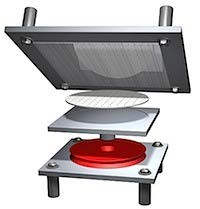
\includegraphics[height=5cm]{discbearing.jpg}
    % \caption{Disc bearing components. (Courtesy R.J. Watson)}
    \caption{圆盘支座组件}
    \label{fig:disc-bearing}
  \end{minipage}%
  \begin{minipage}[b]{0.65\linewidth}
    % \caption{Typical disc bearings. (Courtesy R.J. Watson)}
    \caption{典型圆盘支座}
    \label{fig:typical-disc-bearing}
  \end{minipage}
\end{figure}

% Disc bearings are reasonably economical, but widespread use has been limited because of their originally patented and proprietary status, which made them available only from a single source. Now that there are additional bearing manufacturers that can supply disc bearings, their use has increased.
圆盘支座相当经济,但由于其最初的专利和专有地位,其使用受到限制,这使得它们只能从单一来源获得。现在有更多的支座制造商可以提供圆盘支座,它们的使用也增加了。

% \subsubsection{Spherical/Cylindrical Bearings}
\subsubsection{球面/柱面支座}
% Spherical bearings are used primarily for accommodating large rotations about multiple or unknown axes. Sometimes referred to as curved sliding bearings, spherical bearings permit rotation about any axis, and cylindrical bearings permit rotation about one axis. In these bearing types, rotation is developed by sliding a convex metal surface (lower element) against a concave \acrshort{ptfe} surface (upper element) (see \cref{fig:spherical-bearing}). The rotation occurs about the center of the radius of the curved surface, and the maximum rotation is limited by the geometry and clearances of the bearing. Translational movement is accomplished by incorporating a flat \acrshort{ptfe} sliding surface. Horizontal loads may be partially resisted by the curved geometry of the spherical head, however large horizontal loads may require additional external restraint.
球面支座主要用于适应围绕多个或未知轴的大旋转。有时称为弯曲滑动支座,球面支座允许绕任何轴旋转,而柱面支座允许绕一个轴旋转。 在这些支座类型中,旋转是通过将凸形金属表面(下部元件)相对于凹形 \acrshort{ptfe} 表面(上部元件)滑动来实现的(参见 \cref{fig:spherical-bearing})。 旋转围绕曲面半径的中心发生,最大旋转受支座的几何形状和间隙限制。 平移运动是通过合并一个平坦的\acrlong*{ptfe}滑动表面来完成的。 球形头部的弯曲几何形状可能会部分抵抗水平载荷,但是大的水平载荷可能需要额外的外部约束。

\begin{figure}
  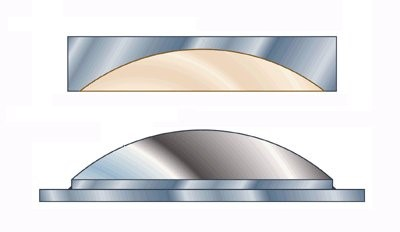
\includegraphics[width=0.6\linewidth]{spherical-bearing.jpg}
  % \caption{Typical spherical bearing. (Courtesy D.S. Brown)}
  \caption{典型球面支座}
  \label{fig:spherical-bearing}
\end{figure}

% Spherical bearings require highly machined fabrication and are more sensitive to the quality of the initial manufacture and installation than other HLMR bearings. Consequently, although they are generally the most expensive HLMR type, their advantage is their ability to accommodate higher gravity loads and rotations.
球面支座需要高度机加工制造,并且比其他\acrlong*{hlmr}支座对初始制造和安装的质量更敏感。 因此,尽管它们通常是最昂贵的 \acrshort*{hlmr} 类型,但它们的优势在于能够适应更高的重力载荷和转动变形。

% \subsection{Fabricated Steel Bearings}
\subsection{装配式钢支座}
% Fabricated steel mechanical bearings have been used for both fixed and expansion conditions (see \cref{fig:fabricated-steel-bearings}), and have been the longest-used of any other bearing type. Many existing bridges have these types of bearings and some states still use them for new construction. When functioning properly, mechanical steel bearings generally provide the closest representation of assumed structural end conditions of all bearing types, and transmit loads through direct metal-to-metal contact. Most fixed bearings rely on a pin or knuckle to allow rotation while restricting translational movement. Rockers, rollers and sliding types are common used expansion bearings. Typically, steel bearings are expensive to fabricate, install and maintain, which in part accounts for their popularity. Further, steel bearings typically provide only uni-directional movement. These types of bearings are fully designed by the engineer to accommodate loads, movements, and rotations, and can be developed to accommodate large requirements.
装配式钢支座已用于固定和扩展条件(参见 \cref{fig:fabricated-steel-bearings}),并且是所有其他支座类型中使用时间最长的。 许多现有的桥梁都有这些类型的支座,一些州仍在将它们用于新建筑。 当正常运行时,机械钢支座通常提供最接近所有支座类型的假定结构最终条件的表示,并通过直接的金属与金属接触传递载荷。 大多数固定支座依靠销或关节来允许旋转,同时限制平移运动。 摇臂式、滚子式和滑动式是常用的膨胀支座。 通常,钢制支座的制造、安装和维护成本很高,这在一定程度上解释了它们的受欢迎程度。 此外,钢支座通常仅提供单向运动。 这些类型的支座完全由工程师设计以适应负载、运动和旋转,并且可以开发以满足更大的要求。

\begin{figure}
  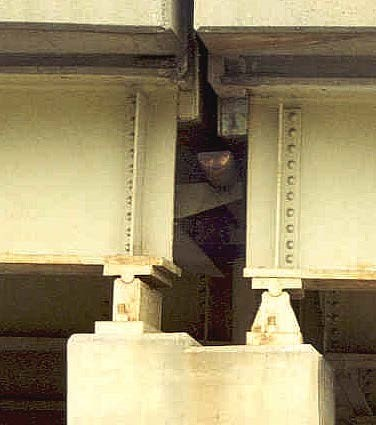
\includegraphics[width=0.5\linewidth]{steel-bearings.jpg}
  % \caption{Fabricated steel bearings—rocker expansion and fixed conditions. (Courtesy HDR)}
  \caption{装配式钢支座——辊轴支座和固定支座}
  \label{fig:fabricated-steel-bearings}
\end{figure}

% Bronze lubricated plate bearings have been used in conjunction with steel bearings to accommodate smaller amounts of movement at expansion ends, but are not used much today. \acrshort{ptfe} sliding surfaces have replaced bronze sliding plates because of a much lower coefficient of friction and lower cost.
青铜润滑板支座已与钢支座结合使用,以适应活动端的较小运动量,但如今使用不多。 因为\acrlong*{ptfe}滑动表面摩擦系数低得多,成本也低得多,它现在已经取代了青铜滑动板。

% \section{Factors Influencing Service Life of Bearings}
\section{影响支座使用寿命的因素}

% This section discusses various factors influencing the service life of bearings utilizing a fault tree analysis approach that first identifies service life issues that generally pertain to all bearing types. This is followed by specific discussions of service life issues pertaining to individual bearing types.
本节使用\gls*{faulttree}分析方法讨论影响支座使用寿命的各种因素,该方法首先确定通常与所有支座类型相关的使用寿命问题。 随后具体讨论了与各个支座类型有关的使用寿命问题。

% \subsection{Factors Affecting Service Life of All Bearing Types—Fault Tree Analysis}
\subsection{影响所有支座类型使用寿命的因素——\glsentrytext{faulttree}分析}

% A general description of the fault tree analysis approach for identifying factors affecting service life is given in \cref{chp:general-frame} on general framework. \cref{chp:bridge-system-selection} on system selection, further applies the fault tree analysis to identify factors affecting service life of overall bridge systems, which includes deck, superstructure, and substructure components. This section applies specific parts of the fault tree analysis to identify service life factors that apply to bearings.
在\cref{chp:general-frame}\nameref{chp:general-frame}中给出了用于识别影响\gls*{servicelife}的因素的\gls*{faulttree}分析方法的一般描述。\cref{chp:bridge-system-selection}在系统选择方面,进一步应用\gls*{faulttree}分析来确定影响整个桥梁\gls*{system}\gls*{servicelife}的因素,包括桥面系、上部结构和下部结构\gls*{component}。 本节应用\gls*{faulttree}分析的特定部分来确定适用于支座的\gls*{servicelife}因素。

% \cref{fig:fault-tree-bearing} shows an overall fault tree diagram that identifies factors affecting service life for bridge bearings. The diagram identifies factors at descending levels that cause or contribute to service life reduction.
\cref{fig:fault-tree-bearing} 显示了一个整体\gls*{faulttree}图,它确定了影响桥梁支座\gls*{servicelife}的因素。 该图确定了导致或导致\gls*{servicelife}缩短的下降级别的因素。

\begin{figure}
  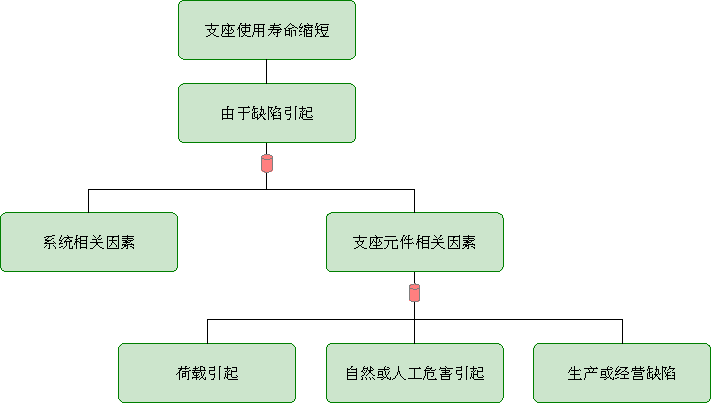
\includegraphics{fault-tree-bearing.pdf}
  % \caption{Fault tree analysis for factors affecting service life of bearings}
  \caption{影响支座寿命因素的\gls*{faulttree}分析}
  \label{fig:fault-tree-bearing}
\end{figure}

% As discussed in \cref{chp:bridge-system-selection}, the first level affecting service life of a bridge system is either obsolescence (relating to function or operation) or deficiency (relating to deterioration or damage). In relation to bearings, however, service life issues are typically caused by deterioration or damage, not by obsolescence, so the fault tree moves directly to deficiency. Following this, deficiencies can be either:
正如\cref{chp:bridge-system-selection}中所讨论的,影响桥梁\gls*{system}\gls*{servicelife}的第一级是\gls*{obsolescence}(与功能或操作有关)或缺陷(与\gls*{deterioration}或损坏有关)。 然而,就支座而言,\gls*{servicelife}问题通常是由\gls*{deterioration}或损坏引起的,而不是由\gls*{obsolescence}引起的,因此\gls*{faulttree}直接移动到缺陷。 在此之后,缺陷可能是:

% \begin{itemize}
%   \item System-related (i.e., related to other items within the bridge system or to the layout of the system); or
%   \item Bearing element related (i.e., related directly to bearing element performance).
% \end{itemize}
\begin{itemize}
  \item \gls*{system}相关(即与桥梁\gls*{system}内的其他项目或\gls*{system}布局相关);
  \item 支座元件相关(即与支座元件性能直接相关)。
\end{itemize}

% Deficiencies can then be subcategorized to that caused by loads, natural or man-made hazards, or production/operation defects.
然后可以将缺陷细分为由荷载、自然或人为危害或生产/运营缺陷引起的缺陷。

% \subsubsection{Deficiency of System-Related Items}
\subsubsection{系统相关项目的不足}

% System-related items whose deficiencies can directly affect bearings are primarily attributed to system production/operation defects, and are illustrated in \cref{fig:system-related-deficiency}.
缺陷直接影响支座的系统相关项目主要归因于系统生产/运营缺陷,并在\cref{fig:system-related-deficiency} 中进行了说明。

\begin{figure}
  % \includegraphics[width=\linewidth]{graphic-file}
  \caption{Bridge system-related deficiencies}
  \label{fig:system-related-deficiency}
\end{figure}

% These factors typically relate to deficiencies in elements, details, and general layout of the overall bridge system that can adversely affect bearing performance. Other types of production/operation defects are discussed in \cref{par:production-defects} as they relate to individual bearing elements.
这些因素通常与可能对支座性能产生不利影响的整个桥梁\gls*{system}的\gls*{element}、细部构造和总体布局方面的缺陷有关。 其他类型的生产/操作缺陷在\cref{par:production-defects}中讨论,因为它们与单个支座元件有关。

\paragraph{桥面伸缩缝漏水}
% Of all system-related deficiencies, leaking deck expansion joints can have the greatest negative impact on bridgebearings. This applies to both open and sealed joints.
在所有与系统相关的缺陷中,桥面伸缩缝漏水对桥梁支座的负面影响最大。 对于开放式和密封式接缝都是如此。

% Open joints, such as finger dams or sliding plate dams, typically allow drainage to pass through and be collected in troughs and below-joint drainage systems. Failure or clogging of these drainage systems allows deck drainage and debris to spill onto all bridge elements below, including bearings.
开放式伸缩缝,例如指状水坝或滑板式水坝,通常允许排水通过并收集在槽和接缝下方的排水系统中。 这些排水系统的故障或堵塞会使桥面板排水和杂物溢出到下面的所有桥梁\gls*{element}上,包括支座。

% Sealed joints, such as compression joints, strip seals, or large modular joints, are intended to prevent deck drainage from spilling through. However, failure or damage to these types of joints can also allow deck drainage to leak through onto bridge elements below.
密封伸缩缝,例如压缩伸缩缝、条形密封件或大型模块化伸缩缝,旨在防止桥面系排水系统溢出。 然而,这些类型的伸缩缝失效或损坏也可能导致桥面系排水泄漏到下面的桥梁\gls*{element}上。

% Bearings located below leaking deck joints—particularly those in northern wet climates—are subject to deck drainage, deicing chemicals, and other deck debris, which is a leading cause of deterioration and reduced service life. Drainage and deicing chemicals cause corrosion of exposed steel elements, and debris buildup affects proper rotation and expansion movement.
位于漏水的桥面板伸缩缝下方的支座——尤其是在北方潮湿气候下的支座——会受到桥面排水、除冰盐和其他桥面杂物的影响,这是导致\gls*{obsolescence}和\gls*{servicelife}缩短的主要原因。排水和除冰盐会导致暴露的钢\gls*{element}腐蚀,杂物堆积会影响适当的转角和伸缩运动。

% \paragraph{Improper Bearing Orientation}
\paragraph{支座方向不当}

% In skewed, curved, and wide bridges, bearings are subjected to multi-directional movements and/or rotations. Improper bearing orientation and/or inadequate multi-direction movement capacity can lead to higher stresses, wear, and reduced service life.
在斜弯桥和桥面宽度较大的桥梁中,支座会受到多向平移和/或转角的影响。支座方向不当和/或多向运动能力不足会导致更高的应力、磨损和使用寿命缩短。

% Bridges wider than three lanes can experience significant transverse thermal movement. Guides and keeper assemblies should be limited to the interior portions of the bridge that do not experience large transverse movements. Bearing details for outer portions on wide bridges should be designed to accommodate transverse movement.
宽度超过三车道的桥梁在温度作用下横向变形明显。导轨和约束组件应限制在不会经历大横向运动的桥的内部部分。 宽桥外部的支座细部构造应设计为适应横向运动。

% In the case of skewed steel bridges, a phenomenon, commonly referred to as layovers exists during construction. The layovers subject the bearings to rotation of the steel girder about longitudinal axis of the girder (twisting of the section). This subjects the bearing to rotation that is not generally considered in design and subjects the bearing to multi-rotation.
在斜钢桥的情况下,在施工过程中存在通常称为中途停留的现象。 中途停留使支座承受钢梁绕钢梁纵轴的旋转(截面扭曲)。 这使支座经受在设计中通常不考虑的旋转并且使支座经受多旋转。

% \paragraph{Inadequate Inspectability}
\paragraph{可检查性不足}
% Proper inspection of bearings during their service life is critical in order to evaluate proper performance, wear, or deterioration. Early detection of problems can allow maintenance or repair before more serious conditions can develop. Shallower bearing types can be difficult to properly inspect, particularly when limited headroom prevents close access. Consideration should be given in overall bridge system design to allow access for proper inspection of bearings.
在支座的{使用寿命}期间对其进行适当检查对于评估适当的性能、磨损或劣化至关重要。 及早发现问题可以在出现更严重的情况之前进行维护或修理。 较浅的支座类型可能难以正确检查,尤其是当净空高度有限而无法近距离接触时。 在整个桥梁系统设计中应考虑允许对支座进行适当检查的通道。

% \paragraph{Inadequate Replaceability}
\paragraph{可替换性不足}

% Regardless of expected service life, bearings are subjected to severe service conditions, and have a high potential for unintended consequences related to improper design, manufacturing, installation, and maintenance that can lead to shorter service lives than other bridge elements. Consideration should be given in the overall bridge system design to allow for easy replacement of bearings with minimal traffic disruption. AASHTO and NSBA provide recommended bearing details that facilitate replacement \cite{aashtonsba2004s}.
无论预期{使用寿命}如何,支座都会承受严酷的使用条件,并且很可能因设计、制造、安装和维护不当而导致意外后果,从而导致{使用寿命}比其他桥梁{元件}短。 在整个桥梁系统设计中应考虑到允许在最小交通中断的情况下轻松更换支座。 AASHTO 和 NSBA 提供了便于更换的推荐支座详细信息 \cite{aashtonsba2004s}。

% \subsubsection{Deficiency of Bearing Related Items}
\subsubsection{支座相关项的不足}
% Reduced service life of bearings is often caused by deficiencies of individual bearing elements themselves. As illustrated previously in \cref{fig:fault-tree-bearing}, bearing deficiency can be caused by loads, natural or man-made hazards, or production/operation defects.
支座使用寿命的缩短通常是由个别支座元件本身的缺陷引起的。 如先前在 \cref{fig:fault-tree-bearing} 中所示,支座缺陷可能由荷载、自然或人为危害以及生产/运营缺陷引起。

% \paragraph{Bearing Deficiency due to Loads}
\paragraph{荷载引起的支座缺陷}
% \cref{fig:faulttree-bearing-load} illustrates factors affecting bearing service life due to loads.
\cref{fig:faulttree-bearing-load} 说明了由于荷载影响支座使用寿命的因素。

\begin{figure}
  % \includegraphics[width=\linewidth]{faulttree-bearing-load}
  \caption{Factors affecting service life due to loads.}
  \label{fig:faulttree-bearing-load}
\end{figure}

% As illustrated, loads can be traffic loads (primarily truck loads), or system-dependent loads (primarily due to thermal activity). Each of these load types can result in element damage due to wear/fatigue or overload.
如图所示,荷载可以是交通负载(主要是卡车荷载)或系统相关荷载(主要是由于温度作用)。 这些荷载类型中的每一种都可能由于磨损/疲劳或超载而导致元件损坏。

% Truck traffic applies direct vertical load to bearings as well as superstructure end rotation and accompanying horizontal translation. Thermal activity applies horizontal and transverse translations and girder end rotation to bearings; however, depending on intended or unintended levels of restraint, thermal activity can also apply significant horizontal load to bearings.
卡车交通对支座以及上部结构端部旋转和伴随的水平平移施加直接垂直载荷。 热活动对支座施加水平和横向平移以及梁端旋转;然而,根据有意或无意的约束水平,热活动也会对支座施加显着的水平载荷。

% Truck traffic produces high frequency, low amplitude cyclic movement at expansion bearings combined with vertical load. Cyclic movement from girder end rotation results in total cumulative movement that is significantly greater than total cumulative movement due to thermal activity. This behavior primarily affects wear of sliding surfaces.
卡车交通会在膨胀支座处产生高频、低振幅的循环运动以及垂直载荷。 来自梁端旋转的循环运动导致总累积运动明显大于由于热活动引起的总累积运动。 这种行为主要影响滑动表面的磨损。

% Other loads such as those due to wind, longitudinal braking, or earthquakes can also apply various vertical and horizontal loads to bearings that must be resisted.
其他载荷,例如由于风、纵向制动或地震引起的载荷,也会对必须承受的支座施加各种垂直和水平载荷。

All of these loads can ultimately result in bearing element fatigue, wear, or overload at various levels depending
on the specific bearing type and make up. For example, elastomeric bearings are subject to element fatigue, and
PTFE sliding surfaces are subject to wear.

Overload, either from heavy truck loads or large thermal movement, in which the bearings experience greater
loads than assumed in design, can also lead to reduced service life. Overload can result in various forms of damage
depending on bearing type.

Incorrect assumptions during the design process can also significantly affect the service life of bearings because
of system restraint. For example, as described in Chapter 8 on jointless bridges, in the case of curved girder bridges,
there might not be a point within structure that can be designated as point of zero movement. Such an assumption can
lead to use of a fixed bearing type, without any capability or allowance for transverse or longitudinal movements.
The end result of such wrong assumption is that the bearing is subjected to actions that cannot be accommodated by
bearing and the development of significant damage to bearing in the process.

Service life applications to specific bearing types are discussed later in this chapter.

\paragraph{Bearing Deficiency due to Natural or Man-Made Hazards}

\cref{fig:faulttree-bearing-hazards} illustrates factors affecting service life due to natural or man-made hazards. For bearings, hazardrelated
deficiencies typically pertain to thermal climates, coastal climates, or chemical environments.

\begin{figure}
  % \includegraphics[width=\linewidth]{faulttree-bearing-hazards}
  \caption{Factors affecting service life due to natural or man-made hazards.}
  \label{fig:faulttree-bearing-hazards}
\end{figure}

Thermal climates pertain to cold and wet climates accompanied by snow and ice that result in high usage of
deicing chemicals on roadways and bridge decks. Bridge bearings are affected by roadway drainage and salts
leaking through expansion joints, or by salt spray rising up from crossed roadways.

Coastal climates are climates near the ocean or other salt water bodies where bridge bearing elements can be
affected by airborne salt spray.

Chemical environments can include environments near chemical or industrial facilities where corrosive airborne
chemicals can affect exposed bearing elements.

Ultimately, these climates or environments can result in exposed steel element corrosion or degradation of other
bearing materials at various levels depending on specific bearing type and make up. More specific environmental
factors are discussed as they relate to individual bearing types later in this chapter.


\paragraph{Bearing Deficiency due to Production/Operation Defects}
\label{par:production-defects}
\cref{fig:faulttree-bearing-operation} illustrates factors affecting service life of bearings due to production/operation defects. For
bearings, these defects can be in any one of four general subcategories:
\begin{itemize}
  \item Design/Detail,
  \item Fabrication/Manufacturing,
  \item Construction, or
  \item Maintenance.
\end{itemize}


\begin{figure}
  % \includegraphics[width=\linewidth]{faulttree-bearing-operation.pdf}
  \caption{Factors affecting service life due to production/operation defects.}
  \label{fig:faulttree-bearing-operation}
\end{figure}

\subparagraph*{Design/Detail}
Improper bearing design and accompanying details can result in significantly reduced service life. Major base
factors include:
\begin{itemize}
    \item Improper Design Parameters——incorrect or improperly computed design values of vertical load, movement,
    and rotation, or combinations thereof. All bearings must be designed for proper superstructure loads, movements, and
    rotations. Improper calculation and application of these parameters at the design stage can result in bearings that are
    subject to excessive rotation, higher stresses, greater wear, and ultimately, reduced service life.
    \item Improper Design Clearances——improper clearances within bearing details to permit proper movement and/or
    rotation. Details with inadequate clearances can cause binding that limits proper movement or rotation, which results
    in higher stress, damage, wear, and reduced service life.
\end{itemize}

\subparagraph{Fabrication/Manufacturing}
Material or fabrication flaws can lead to performance failure and reduced service life. Proper quality assurance
(QA) and quality control (QC) procedures in accordance with current AASHTO LRFD Construction Specifications
must be implemented in the fabrication or manufacturing of bridge bearings to ensure that the completed bearings
meet specifications and provide required levels of performance (AASHTO 2010). See Section 10.4.1.2.3b for
additional discussion.

\subparagraph{Construction}
Production/operation defects at the construction stage can be due to either element damage or improper
placement. Protective care must be taken during field construction to prevent damage or contamination to sensitive
bearing parts such as sliding surfaces or elastomeric pads or discs. Bearings must be set in the field at proper
positions to accommodate installation temperatures and rotations.

\subparagraph{Maintenance}
Lack of or inadequate bearing maintenance can also lead to reduced service life. Issues typically relate to lack of
cleaning, which results in debris build up below deck expansion joints, and steel element corrosion. Other types of
maintenance related issues are discussed later for specific bearing types. Dirt and debris build up prevents proper
bearing movement and rotation. Debris build up also retains and holds moisture and salt against exposed steel
elements, which leads to corrosion if not cleaned.

\subsection{Factors Affecting Service Life Unique To Each Bearing Type}
This section looks at specific service life issues pertaining to bearing types described in Section 10.2 and addressed within the general fault tree categories described in Section 10.3.1.
\subsubsection{Steel-Reinforced Elastomeric (SRE) Bearings}
Steel reinforced elastomeric bearings have been in service in the United States for over 50 years, and longer elsewhere in the world, with very good results. They are typically very robust, and of all bearing types they likely have the best chance for achieving a service life greater than 100 years. When properly designed, manufactured, and installed, there is very little that can go wrong, and long-term maintenance requirements are minimal. In rare instances however, certain problems have been observed, most often associated with production/operation defects relating to design and manufacturing.

\paragraph{Improper Design}
In rare occurrences, improper design has led to overloaded pads, or pads subjected to excessive lateral movement, causing excessive bulging, splitting, or delamination. The following describes various potential failure modes and other issues with elastomeric bearings, and how they are addressed within current AASHTO design provisions. A significant amount of research has been performed on SRE bearings, and designs that follow recent provisions in the LRFD Specifications should adequately avoid these issues as they would affect service life.


\subparagraph{Shear Deformation}
Elastomeric bearings accommodate longitudinal and transverse expansion and contraction by shear deformation
within the elastomer itself. If the shear displacements of the bearing are large, they may cause some rollover at the
acute ends of the layer, which leads to cracking in the elastomer at the end of the top and bottom reinforcement
plates. This condition is exacerbated by cyclic loading. Fatigue tests simulating temperature movement, which is
low-cycle, high-amplitude movement, indicate that keeping the shear strain below 0.5 will prevent this. This is not
conservative, however, if the deformation is due to high-cycle loading caused by braking forces or end rotation. It
was found that high cycle fatigue was more damaging, and in those cases the maximum shear strain should be limited
to 0.10. (Roeder et al. 1990)


\subparagraph{Plate Delamination and Debonding:}
Shear delamination between layers of elastomer and steel reinforcing plates is the most significant potential
mode of failure. Large shear strains occur in elastomeric bearings due to combined axial load, rotation, and shear, and are illustrated in \cref{fig:deformation-elastomeric-bearing} (Stanton et al. 2008). Each of these shear strains reaches its maximum value at the
same location, namely the very edge of the layer at which the elastomer is bonded to the reinforcing plate. Under
severe loading, this condition leads to local detachment and debonding of the elastomer from the plate. Once
debonding occurs, the elastomer starts to extrude from the bearing, which in turn causes significant vertical
deflection. Further, cyclic shear strain causes additional debonding damage than static shear strain of the same
magnitude. Section 14.7.5.3.3 of the LRFD Specifications provides updated (2010) requirements for considering
shear strain caused by combined axial load, rotation, and shear displacement, and considers an amplification factor of
1.75 for combined shear strains due to cyclic loading caused by traffic.

\begin{figure}
  % \includegraphics[width=\linewidth]{graphic-file}
  \caption{Deformations of a laminated elastomeric bearing layer. (Stanton et al. 2008)}
  \label{fig:deformation-elastomeric-bearing}
\end{figure}

\subparagraph{Instability}
Large lateral movement combined with large end rotations results in thick bearing designs. If the bearing
becomes thick enough, instability can affect its performance (Stanton et al. 2008). The layered construction and the
very low shear modulus of the rubber combine to cause this potential problem. Quite often the bearing is made as
wide as possible (transverse to the girder axis) and then only a short length is needed to provide sufficient bearing
area for supporting the axial load. However, too short a length would again risk instability. In such bearings, the axial
stress may therefore be significantly lower than the limit because of the indirect influence of stability requirements.
Section 14.7.5.3.4 of the LRFD Specifications provides updated (2010) requirements for stability, and limits the
average compression stress to half the predicted buckling stress.

\subparagraph{Plate Fracture}

Lateral expansion of the elastomeric layers causes tension in the steel reinforcing plates (Stanton et al. 2008). At
extreme loads the plates could fracture, typically splitting along the longitudinal axis of the bearing. However, in
plates of the thickness currently used, this behavior does not occur until the load has reached five to 10 times its
design value, so plate fracture seldom controls design. Plates could actually be thinner but they are typically sized in
practice to keep them from bending during the molding process. Section 14.7.5.3.5 of the LRFD Specifications
provides requirements for the thickness of steel reinforcement, and considers both strength and fatigue.

\subparagraph{Compressive Deflection}

Instantaneous compressive deflection is limited by the Specifications in order to avoid damage to deck joints and
seals, and to avoid additional impact when traffic passes from one girder to the other across a joint. A maximum
relative live load deflection across a joint of 1/8 in. is recommended. Section 14.7.5.3.6 of the LRFD Specifications
provides requirements for compressive deflection.

\paragraph{Improper Fabrication/Manufacturing and Installation}
In addition to proper design, it is imperative that proper manufacturing and installation also be performed, and
effective quality control during these processes is essential for successful performance.

One of the most commonly reported field problems associated with elastomeric bearings, albeit in only few
instances, has been walking out, or slipping from the original position under the girder. Slippage was occurring
primarily in elastomeric pads made of natural rubber because of paraffin that was added during the manufacturing
process in order to meet required ozone degradation requirements established by AASHTO. Neoprene pads have
inherently greater ozone resistance and do not need wax additives. When used, these waxes over time will bleed to
the bearing surfaces and drastically reduce the coefficient of friction between the bearing and its contact surface,
which leads to slipping (Chen and Yura 1995). Use of positive attachment to the substructure or superstructure, such
as bonding, is recommended to prevent this occurrence. However, caution needs to be exercised in bonding
elastomeric pads and contact surface in highly skewed steel bridges because of layovers.

\subsubsection{Cotton Duck Pads (CDP)}
Cotton duck pads are only used by a few states so their performance history is limited. Like SRE bearings,
potential service life issues for CDP are most often associated with production/operation defects and CDPs require
proper design, manufacturing, installation, and maintenance.

For SRE bearings, longitudinal and transverse movements of bridge are accommodated by shear deformation of
the elastomer and the reinforcement has little influence on the shear stiffness of the bearing. CDPs behave differently.
The fabric layers of CDP are many and closely spaced, and result in significantly larger shear stiffness and smaller
shear deformation capacity than in other elastomeric bearing types. As a consequence, CDP tolerate large
compressive stresses, but limited shear deformation because interlayer splitting occurs at much smaller shear strains.
Also, the large shear stiffness of CDP can result in slip of the girder on the CDP, which may result in abrasion and
deterioration of the CDP. As a consequence, translational shear strain is limited to only about 10%. That is, the shear
deflection is limited to only 1/10 of the total CDP thickness. Larger movement requirements with CDP must be
accommodated by the addition of a sliding surface such as \acrshort{ptfe} sliding surface (Lehman et al. 2003).

The stiffness and deformation capacity of CDP varies from manufacturer to manufacturer. Proper quality control
testing is necessary to assure that the bearing pad provides adequate performance.

Delamination of elastomer layers or secretion of oil and wax from the CDP are the common serviceability limit
states for CDP. To control delamination, compressive stress limits of 3000 psi for total dead plus live load and 2000
psi for live load are recommended. Dynamic or cyclic rotation, which induces uplift or partial separation of the pad
from the load surface, may cause delamination and reduced service life. Uplift damage depends on the maximum
total rotation, as well as the rotation range caused by the live load variation, and separate rotation limits are provided.
LRFD Specifications now include design provisions to ensure the serviceability and durability of CDP.

\subsubsection{Sliding Surfaces (Primary Sliding Surfaces, Not Guide Bars)}
Factors affecting service life of bearing sliding surfaces most often relate to deficiencies caused by loads,
including both traffic (truck load) and system-induced (thermal movement). These can result in sliding element wear
(from cyclic movement) and creep or cold flow (from compressive overload).

Deficiencies caused by production/operation defects can also occur, primarily during manufacturing and
construction. They typically relate to surface scratching and damage due to inadequate protection during shipping or
installation. Surface damage leads to increased wear. These problems can be mitigated by proper protection and
inspection during shipping and installation.

Inadequate maintenance, particularly below open or leaking deck expansion joints, can allow buildup of dirt and
other debris that can cause contamination of sliding surfaces and increased wear. Periodic maintenance and cleaning
in these areas can mitigate these problems.

\paragraph{Wear of Sliding Surfaces}
Plain \acrshort{ptfe} is most commonly used for bearing sliding surfaces. It wears under service conditions and may
require replacement after a period of time. Low temperatures, fast sliding speeds, high contact pressures, rough
mating surfaces, and contamination of the sliding interface increase the wear rate. However, fast sliding speed has
been shown to be the more dominant parameter (Stanton, et al. 1999). Movement due to temperature change is lowcycle,
high-amplitude movement, with a slow movement rate, and produces the least amount of wear. However,
movement due to truck load and associated dynamic effects is high-cycle, low-amplitude movement and has a much
faster sliding speed, by as much as a factor of 10. Wear rates associated with high sliding speeds can be as much as
150+ times greater than wear rates at lower sliding speeds. Thus, plain \acrshort{ptfe} should not be used as a sliding surface
for bearings subject to relatively high sliding speeds and low temperatures.

Relatively thin layers of \acrshort{ptfe}, from 1/16 in. to 3/16 in., are commonly used in the United States, but engineers
in other countries often use thicker \acrshort{ptfe} layers to accommodate wear.

Woven or glass filled \acrshort{ptfe} surfaces provide much higher overall wear resistance, especially at higher sliding
speeds, but these surfaces have higher friction coefficients that must be taken into account in the bridge system
design.

Dimpled and lubricated \acrshort{ptfe} also provides exceptional wear resistance and low friction, but the long-term
effectiveness of lubrication is questionable (Stanton et al. 1999).

\msm has been shown to provide exceptional wear resistance, but when used in a dry condition (without
lubrication) it has a much higher friction coefficient than plain \acrshort{ptfe}. When used in a dimpled and lubricated
condition however, its friction coefficient reduces considerably and is more comparable to lubricated \acrshort{ptfe}.

\paragraph{Creep or Cold Flow}
\acrshort{ptfe} may creep (or cold flow) laterally when subjected to high compressive stress and shorten the life of the
bearing. The reduction in \acrshort{ptfe} thickness may also allow hard contact between metal components. Thus, while the
compressive stress should be high to reduce friction, it must also be limited to control creep. \acrshort{ptfe} is frequently
recessed for one half its thickness and bonded to control creep and permit larger compressive stress.

Filled \acrshort{ptfe}, which is reinforced with fiberglass or carbon fibers, has significantly greater resistance to creep,
and is sometimes used to resist creep or cold flow.

\subsubsection{HLMR Pot Bearings}

In past years, pot bearings have had service life problems most often associated with production/operation
defects relating to design and manufacturing. These issues have ultimately resulted in broken internal seals, leakage
or extrusion of the elastomer, abraded elastomeric pads, and metal-to-metal contact, which have led some state
departments of transportation (DOT) to recommend avoiding pot bearings altogether. However, improved design
specifications and tighter manufacturing tolerances developed in the late 1990s have greatly improved overall
performance. Current LRFD Specifications (2012) now incorporate research findings reported in NCHRP Report 432,
High-Load Multi-Rotational Bridge Bearings, 1999, by Stanton, Roeder, and Campbell (Stanton et al. 1999), and
address specific past service life issues. The following items have been recommended to mitigate certain past
deficiencies, and are now part of standard design and manufacturing practice:

\begin{itemize}
  \item Rotational capacity of pot bearings is limited by the clearance between various elements of the pot, piston,
  sliding surface, guides, and restraints (Stanton et al. 1999). Inadequate clearances can cause binding between
  metal components. See \cref{fig:critical-clearances}. Clearance requirements are now included in the specifications.
  
  \begin{figure}
    % \includegraphics[width=\linewidth]{graphic-file}
    \caption{Critical clearances affecting rotation capacity.}\label{fig:critical-clearances}
  \end{figure}
  \item Thickness of the elastomeric pad also affects rotational capacity, and is currently controlled by a 15\% strain
  limit on the pad edge deflection under rotation. This strain value is based more on past practice than research
  results, but it is believed to be a reasonable value.
  \item Pot bearings are able to sustain many cycles of small rotation better than a smaller number of large rotation
  cycles. This is believed to be true because smaller rotations cause deformation of the elastomer but little slip.
  Slip caused by larger rotations abrades the surface of the elastomer. In an attempt to account for this, pot
  bearings should be designed for larger minimum rotations that reduce the potential for over-rotation. This
  minimum rotation should reflect increased rotation caused by construction tolerances expected in practice.
  Further, greater emphasis should be placed on calculation of rotations due to service loads, construction
  loads, and environmental conditions.
  \item Rotational resistance, wear, and abrasion are significantly reduced with a smooth surface finish inside the pot
  and on the piston. Metalizing of these interior surfaces for corrosion protection causes a rougher surface that
  leads to increased damage under cyclic rotation, and should not be used unless buffed to a smooth finish. In
  extreme corrosive environments, stainless steel could be considered.
  \item Failure of sealing rings causing escape of elastomer has been one of the major service life issues with pot
  bearings in past years. Solid circular cross section brass rings and multiple flat brass rings have both been
  used, and each has advantages and limitations. Circular cross section rings provide a tight seal but are
  susceptible to wear under cyclic rotation. Flat rings appear to be more susceptible to leakage and ring
  fracture, but they experience less wear. Heavier flat brass rings have been suggested as a means of improving
  their performance. The performance of circular rings could also be improved if the friction and wear were
  reduced. Currently, both circular cross section and flat brass rings are permitted in the specifications.
  Current design and manufacturing in accordance with LRFD Specifications have greatly resolved past issues
  with sealing rings and leakage of elastomer.
  \item Silicon grease lubrication appears to reduce the wear noted on rings, pot walls, and piston, and is
  recommended for use. This lubrication does not reduce the ultimate wear of the elastomeric disc.
  \item Relatively small lateral load (5\% of gravity load) when combined with cyclic rotation can dramatically
  increase the rotational resistance, wear, and leakage of pot bearings. This damage is caused by the piston rim
  dragging against the pot wall during rotation. Alternate methods of external restraint are recommended for
  large lateral loads to mitigate this damage potential.
  \item Dirt or contamination in the pot increases wear and abrasion of the rings, pot, and elastomeric disc, and
  increases the potential of elastomer leakage. To mitigate this potential, pot bearings need to be sealed and
  protected during shipping and installation.
\end{itemize}

Although newer design and manufacturing criteria have improved the overall performance of pot bearings in
recent years, it is still recognized that this bearing type has internal moving parts subject to wear and abrasion that
can lead to reduced service life. Newer requirements for long-term deterioration testing in accordance with current
AASHTO Construction Specifications provide greater assurance of proper performance.

\subsubsection{HLMR Disc Bearings}
Since their first use in the early 1970s, these bearings have had good performance and few reported field
problems. Potential service life problems (albeit few) would most likely be associated with production/operation defects relating to design and manufacturing. Current specifications are minimal regarding design, and are generally
performance related. Therefore, performance testing and manufacturing QC measures are necessary to verify
compliance.

Previous research testing of disc bearings for combined load and rotation (Stanton et al. 1999) made several
performance conclusions:

\begin{itemize}
  \item Tests showed that rotation of disc bearings is partly accommodated by uplift of the steel plates from the
  urethane disc, especially if the compressive load is light. This should not result in any problems with fixed
  bearings, but could be a concern with sliding bearings, since uplift of the disc produces edge loading on the
  \acrshort{ptfe} sliding surface. To mitigate this potential problem, LRFD Specifications limit the edge contact stress
  on \acrshort{ptfe} surfaces and AASHTO Construction Specifications require proof load testing.
  \item Tests showed the urethane disc to be somewhat deformed and abraded by cyclic rotations, but the damage
  was not so severe as to affect the performance of the bearing. AASHTO Construction Specifications require
  cyclic deterioration testing to confirm long-term performance.
\end{itemize}


\subsubsection{HLMR Spherical Bearings}
Although a very robust system, these types have had service life problems, most often associated with
production/operation defects relating to design and manufacturing. The difficulties appeared to be attributable to
faulty fabrication by manufacturers that were not necessarily first-tier suppliers. These bearing types require very
precise manufacturing tolerances to assure proper fit of the curved mating surfaces.

Rotation capacity can be set at almost any desired level provided adequate clearances are provided.

\acrshort{ptfe} surfaces may also eventually wear out. Variations in friction with different types of \acrshort{ptfe} and under
different temperature and load conditions cause variations in behavior that can lead to performance issues. Woven
\acrshort{ptfe} has often been used with spherical bearings in the United States, while dimpled and lubricated \acrshort{ptfe} is often
used in Canada and Europe.

These types of bearings are typically larger than other types and generally require additional space. Spherical
bearings are traditionally considered to be the most expensive HLMR bearing type, but are also traditionally
considered the most reliable.

\subsubsection{Fabricated Mechanical Steel Bearings}

Fabricated mechanical steel bearings have been used for the longest time of any bearing type and have the
potential for extended service life if properly protected and maintained. Factors affecting service life relate to several
categories including loads, primarily overload, which results in binding or over-rotation of rocker bearings; natural
or manmade hazards, which result in steel element corrosion; and production/operation defects, specifically due to
lack of maintenance.

Fabricated mechanical steel bearings have been used for the longest time of any bearing type and have the
potential for extended service life if properly protected and maintained. Factors affecting service life relate to several
categories including loads, primarily overload, which results in binding or over-rotation of rocker bearings; natural
or manmade hazards, which result in steel element corrosion; and production/operation defects, specifically due to
lack of maintenance.

\paragraph{Loads}
Rocker expansion bearings can be designed for wide ranges of movement, but can have limited potential for
accommodating overload. Excessive translation can lead to rockers tipping over, which has been reported in a few
instances.

\paragraph{Natural or Man-Made Hazards}
Corrosion of steel bearings, particularly those located below open or leaking deck joints in thermal environments,
is the highest cause of reduced service life for these bearing types. In these locations, steel bearings are highly
susceptible to corrosion due to roadway drainage with deicing salts and other dirt accumulation. Coastal climates and
other chemical environments are also catalysts for steel element corrosion.

Pin, roller, and rocker bearings have direct metal-to-metal contact, which creates an environment of high stress
concentration and accumulation of moisture between surfaces. In the areas of contact, any protective coating on the
steel is inevitably damaged by the relative movement. All of these conditions contribute to corrosion.

Corroded expansion bearings can lockup or freeze, subjecting beams and substructure elements below to
additional load and potential damage. Fyfe et al. 2006, reported that steel rocker and roller bearings are the most
susceptible to freezing in position along with older type metal sliding plates. When bearings are frozen, bridges
develop their own provisions for contraction and expansion, such as pier cap cracking or rocking of piers or
abutments.

Dirt and debris accumulation has caused some rocker-type expansion bearings to move beyond their limits and
actually roll over causing the superstructure to drop several in. or more. Figure 10.16 illustrates a ratcheting effect
reported by Modjeski and Masters in 2008, whereby rocker bearings at one pier on the Birmingham Bridge in Pittsburgh, Pennsylvania tipped over because of corrosion and debris accumulation. The rockers had an initial lean,
and a leaking expansion joint above caused corrosion and increasing accumulation of debris on the bearings and
under one side of the rockers. A ratcheting effect followed whereby additional debris and corrosion material kept
accumulating under the rockers causing additional and increasing tilt. This continued until a lateral force or kick
developed against the pier cap, which caused the pier to move just enough to initiate the final tipping of the rocker
bearings.

Steel rocker bearings have also performed poorly in seismic events and have been replaced as part of seismic
retrofit in many instances.

\begin{figure}
  % \includegraphics[width=\linewidth]{graphic-file}
  \caption{Ratcheting effect caused by debris and corrosion. (Modjeski and Masters 2008)}\label{fig:ratchet-debris-corrosion}
\end{figure}

\paragraph{Production/Operation Defects}
Lack of maintenance has been a contributing factor to reduced service life for steel bearings in many instances.
Coating loss, surface corrosion, and debris buildup, all of which lead to reduced service life, can be effectively
mitigated by periodic maintenance if performed. In locations below open deck expansion joints, particularly in
thermal environments where bearings are highly susceptible to roadway drainage, salt, and debris, periodic cleaning
to prevent buildup of deleterious materials is essential.

\section{Options for Enhancing Service Life of Bearings}
This section presents available options for mitigating various bearing service life issues that were identified in
Section 10.3. A procedure to select the optimal bearing type for given loads, movements, and environmental
conditions is presented in Section 10.5.

Options for enhancing service life of bearings are presented in a way that addresses the issues discussed in the
fault tree analysis and the specific categories and sub-categories of deficiencies that were shown to cause damage or
deterioration. As previously illustrated, bearing deficiencies can be either related to bridge system deficiencies or
related directly to bearing element deficiencies. Deficiencies can then be attributed to those caused by loads, natural
or man-made hazards, or production/operation defects

In the discussion of available options for enhancing service life of individual bearing types, the following general
solution categories are included and addressed as applicable:

\begin{itemize}
  \item Avoidance eliminates or bypasses a particular service life issue. This is a primary consideration, and should
  be incorporated where possible.
  \item Mitigation improves performance through enhanced materials, greater protection, or effective maintenance.
  Where avoidance is not practicable, mitigation techniques should be implemented to improve service life.
  \item Acceptance considers that a particular bearing or bearing component may not be able to achieve a service life
  equal to the bridge system design service life, even after mitigation to improve its service life, and may
  eventually need to be replaced.
\end{itemize}

In many instances, the need to provide capabilities and details for easy bearing replacement may still be a
necessary consideration because of uncertainties regarding loads, hazards, or production/operation defects that can
cause premature service life issues.

\subsection{General Options for All Bearing Types}
\subsubsection{Solutions for Deficiencies of System-Related Items}
The following table summarizes solutions for various service life issues identified in Section 10.3.1.1, and briefly
identifies what each solution provides and what other considerations may still be needed. System-related issues were primarily due to production/operational defects and, more specifically, due to design and details of components
within the overall bridge system. Further discussion relating to each issue follows this table.

\begin{table}
  \caption{Solutions for Service Life Problems–All Bearing Types.}
  \label{tab:solution-all-bearing}
  % \input{tables/filename}
\end{table}


\paragraph{Leaking Deck Joints}
The following are possible solutions for avoiding or mitigating bearing damage or deterioration caused by
leaking deck joints. In considering options for improving service life, avoiding deck expansion joints by using
continuous systems and/or integral systems offers the best opportunity. Where possible, integral systems that
eliminate bearings entirely should also be considered, but in most cases this will not be feasible or practical, and use
of bearings cannot be avoided.

\begin{itemize}
  \item Integral abutment systems that avoid deck joints and bearings. Refer to Chapter 8 on jointless bridges, for
  general design guidelines. This has become a popular approach by many states for improving bridge service
  life. Fully-integral abutment construction eliminates both deck joints and bearings at abutments, and is also
  lower in initial cost. Semi-integral construction eliminates deck joints.
  \item Proper use of integral abutments requires an understanding of pile and cap behavior and limitations regarding
  bridge length and geometrics such as curvature and skew.
  \item Integral pier systems that avoid deck joints and bearings. See Chapter 2 on system selection, for more
  detailed discussion of integral pier options.
  \item Bridge systems using integral girder/pier cap construction have been used occasionally by some states to
  accommodate vertical clearance issues, to avoid sharp skews, or to develop frame action for seismic design.
  But they can also serve to eliminate joints, bearings, and associated future maintenance. Although there is a
  higher initial structure cost, savings are realized with integral pier caps in lower approach fills and lower
  long-term maintenance.
  \item Cast-in-place, post-tensioned integral bent caps have been used for many years, but are not widely employed.
  The Tennessee Department of Transportation (DOT) had its first application in 1978, with several others
  since, and all have performed well. The concept allows main longitudinal girders to pass directly through the
  pier’s cap, rather than over the top in the traditional manner.
  \item Integral caps can also maximize column efficiency. Frame action in the longitudinal direction reduces
  column design moments at column bases compared to conventional cantilever columns, and can also enhance seismic performance. However, it must also be considered that integral pier columns may also need to resist
  additional longitudinal moments due to live load, and a system analysis is required.
  \item When multiple piers are made integral with the superstructure, expansion must be accommodated by flexure
  of the pier columns. Tall, slender columns are best suited for this type of construction because their greater
  flexibility can accommodate temperature movement with less force developed.
  \item Continuous superstructure systems that avoid or minimize number of deck joints. These systems include
  fully-continuous, continuous for live load, or continuous deck slabs (link slab). These continuous systems
  can be combined with either integral abutments or conventional abutments. Bearings are still utilized at
  piers, but are protected by continuous superstructure.
  \item Mitigate for bearings below deck joints. When bearings must be located below deck expansion joints,
  mitigation procedures should be implemented. Depending on the environmental severity, all exposed steel
  bearing parts, which also includes sole plates, masonry plates, guides, and anchor bolts, should be stainless
  steel, galvanized, or metalized. These areas should also be cleaned periodically as part of a regular
  maintenance program to prevent salt and debris build up.
  \item Mitigate by repairing or replacing leaking joints. In existing bridges with deck joints, a cost effective
  strategy is to repair or replace joints when they start to leak, which would prevent any deterioration below the
  joint. This proactive approach to preventative maintenance requires periodic inspection with immediate
  repair or replacement when necessary.
\end{itemize}

\paragraph{Improper Expansion-Bearing Orientation}
Proper orientation of bearings in curved and skewed bridges, which are subjected to multi-directional movements
and/or rotations should be provided. Improper bearing orientation and/or multi-directional movement demand can
lead to higher stresses, damage, wear, and reduced service life.

\begin{itemize}
  \item Curved girder bridges. These bridges do not expand and contract along girder lines. A typical approach is
  to assume movement to occur along chord lines from the fixed point to expansion points. See \cref{fig:bearing-orientation-curved}. See Chapter 8 on jointless bridges for additional discussion on determining the point of zero movement or
  fixed point in integral abutment bridges.

  \begin{figure}
    % \includegraphics[width=\linewidth]{graphic-file}
    \caption{Recommended bearing orientation on a horizontally curved alignment. (Courtesy NSBA)}\label{fig:bearing-orientation-curved}
  \end{figure}
  \item Large skew bridges. For these bridges, one approximate solution is to consider the major axis of thermal
  movement along the diagonal from the acute deck corners due to thermal movement of the bridge deck. The
  alignment of bearings should be parallel to that axis. See \cref{fig:bearing-orientation-skew}. It is necessary for expansion
  bearings to have multi-directional capabilities.
  
  \begin{figure}
    % \includegraphics[width=\linewidth]{graphic-file}
    \caption{Recommended bearing orientation for large skew bridges. (Courtesy NSBA)}\label{fig:bearing-orientation-skew}
  \end{figure}
  \item Wide Bridges. Bridges wider than three lanes can experience significant transverse thermal movement.
Guides and keeper assemblies should be limited to the interior portions of the bridge that do not experience
large transverse movements. Bearing details for outer portions on wide bridges should be designed to
accommodate transverse movement combined with longitudinal movement.
\end{itemize}

\paragraph{Proper Access for Bearing Inspection}
Details, particularly sufficient room and access at tops of piers and abutments to permit proper bearing
inspection, should be provided. Early detection of bearing related issues can allow maintenance or repair before
major service life-reducing events can develop. When possible, shallow bearings should be placed on pedestals at tops of piers and abutments in order to provide greater clearance for inspection. Use of thicker sole plates can also
help provide greater clearance.

\paragraph{Proper Capability for Bearing Replacement}
Details that will accommodate the potential need for replacement of all or part of the bearing system should be
provided with the following considerations:
\begin{itemize}
  \item Jacking locations should be provided at every girder. An alternative is to provide for jacking under a
  diaphragm that lifts adjacent girders simultaneously.
  \item Bearing attachment details should allow ease of replacement. If the bearing is unattached, it can easily be
  pulled from its position when the load is removed. Welds can be cut, but doing so requires equipment that
  may be cumbersome in the space available. Grinding may also be needed to produce a flat enough surface for
  installing the new bearing. Any anchor bolts should be placed so that they do not impede the removal of the
  bearing.
  \item Bearings should be detailed in a way that they can be replaced with only 1/4 in. of jacking to avoid causing a
  bump at the top of the deck that would affect traffic. The details also need to provide adequate vertical
  clearance for jacking. Jacking points on the structure should be designed to accommodate both dead load
  and live load in order to be able to maintain traffic during bearing replacement. (Actual jacking loads may
  have to include a factor applied to the design load to break loose the component before lifting.) Jacking for
  elastomeric bearings needs to consider the effect of compressive dead load strain in determining the amount
  of lift.
\end{itemize}

\subsubsection{Solutions for Bearing Related Deficiencies}
\paragraph{Due to Loads—Traffic- and System-Dependent}
Service life issues can be avoided by:

\begin{itemize}
  \item Determining truck traffic-induced cyclic movement for consideration in particular bearing type design, or
  \item Determining proper levels and combinations of load, movement and rotation.
\end{itemize}

\paragraph{Due to Natural or Man-Made Hazards}
The potential for steel element corrosion should be avoided by using stainless steel, or mitigated by high
performance protective coatings (galvanizing or metalizing).

\paragraph{Due to Production/Operation Defects}
\subparagraph{Design/Detail Related}
\begin{itemize}
  \item Proper Loads, Movement, and Rotation
  
  Design should take into account proper levels and possible combinations of load, movement, and rotation in order to avoid problems due to excessive stress, translation or over-rotation. A considerable number of bearing failures are attributed to improper allowance for displacements.

  Further, construction tolerances and possible construction loadings, and how they might affect bearing loads and movements should also be considered. It is recommended that the worst possible combination of loads and displacements due to construction tolerances be considered. In other words, design displacements should include the largest sum of displacements caused by the worst out of level placement of piers and abutments, the largest camber and deflection, and the most adverse tolerances permissible in the construction of the bridge and bearing.

  In AASHTO/NSBA Steel Bridge Collaboration—Steel Bridge Bearing Design and Detailing Guidelines, published in 2004, Appendix A provides recommendations for calculating beam rotations for dead load and live load conditions. There is great variation in the methods used in the industry for calculating live load rotations, and the guide was developed based on methods used in several states. A realistic approach for computing beam rotations is presented in the NSBA guideline.
  \item Proper Clearances
  
  Adequate clearances should be provided for horizontal movement and rotation to prevent binding, wear, or damage to restraining devices, anchor bolts, or internal bearing elements. Adequate widths and clearances at pier and abutment bridge seats should be provided to allow for required movement and rotation.
\end{itemize}

\subparagraph{Fabrication/Manufacturing Related}
Proper QA/QC procedures in the fabrication or manufacturing of bridge bearings are essential to assure that the
completed bearings meet specifications and provide the required levels of performance. Current AASHTO LRFD Construction Specifications provide minimum requirements for packaging, handling and storage, fabrication
tolerances, materials and general performance. Testing requirements include: material certification tests, material
friction tests, dimension checks, clearance tests, bearing friction tests, long term deterioration tests, proof load tests,
and horizontal force capacity tests. The specifications require that manufacturers provide certification that each
bearing satisfies the requirements of the contract drawings and construction specifications.

\subparagraph{Construction Related}
Care and protection during field construction should be provided in order to prevent damage to protective
coatings or damage/contamination to sensitive bearing parts such as sliding surfaces or elastomeric pads or discs.

Proper QA/QC procedures should be provided during construction to assure that bearings are initially set with
specified position, clearances and rotation.

\subparagraph{Maintenance Related}
Periodic maintenance cleaning should be provided at intervals depending on the location within the bridge
system and environmental hazard conditions to avoid debris build up that could affect movement and rotation
performance.

Steel surface cleaning and coating maintenance should be provided in order to prevent corrosion of exposed steel
elements.


\subsection{Options Related to Specific Bearing Types}

\subsubsection{Elastomeric Bearings—Plain and Steel Reinforced}
The following technology table summarizes solutions for various service life issues identified in Section 10.3.2.1
for elastomeric bearings, and briefly identifies the advantages and disadvantages of each solution. Problems with
elastomeric bearings, albeit rare, have been associated with production/operational defects relating to design,
manufacturing, and installation. Following this table is further discussion relating to each issue.

\begin{table}
  \caption{Solutions for Service Life Problems—Elastomeric Bearings}
  \label{tab:solutions-elastomeric-bearing}
  % \input{tables/solutions-elastomeric-bearing}
\end{table}

\paragraph{Improper Element Design Resulting in Excessive Shear Deformation and Excessive Bulging, Splitting, or Delamination}
These problems can be avoided by following recent provisions (2010) in the LRFD Specifications for either
Method A or B. As previously discussed, improper design has, in some instances, resulted in deficiencies. Extensive
research has identified various failure modes when pads are subjected to excessive shear deformation or overload.
See Section 10.3.2.1.1 for further discussion of failure modes.

\paragraph{Need for Greater Longitudinal Movement Capacity}
When there is a need to accommodate large displacements along with smaller axial loads, such as might be found
at the end spans of a long continuous bridge, the use of a low-profile elastomeric bearing combined with a PTFE or higher performing sliding surface offers a practical solution. In these cases, cyclic end movement due to girder
rotation caused by truck load can cause PTFE surface wear. This can be avoided by designing the elastomeric pad to
accommodate rotation and the smaller cyclic movement due to truck loads, and the sliding surface to accommodate
the larger longitudinal movement due to thermal load.


\paragraph{Need to Accommodate Multi-Direction Complex Movement}
When movement direction is not readily determined, such as with curved or skewed bridges, use of circular pads
can more easily accommodate multi-directional requirements. Circular pads typically offer an advantage by requiring
narrower bridge seats than rectangular pads when placed on a skew; however, circular pads are not as efficient from a
design standpoint as properly oriented rectangular pads.

\paragraph{Slipping or Walking Out}
This can be avoided with the following solutions:
\begin{itemize}
  \item Limiting use of wax additives in the manufacturing of the elastomer. This prevents or reduces future bleeding of the wax to the contact surface, which results in a much lower coefficient of friction and bearing slipping.
  \item Providing positive attachment of the elastomeric pad to the bearing sole plates.
\end{itemize}

\paragraph{Improper Fabrication/Manufacturing}
Effective quality control during manufacture is essential for successful performance. Proper cleanliness and care
during fabrication helps prevent debonding of reinforcing plates with elastomer.

\subsubsection{Cotton Duck Pads (CDP)}
The following technology table summarizes solutions for various service life issues identified in Section 10.3.2.2
for CDPs. These bearing types have performed well, but have had limited usage. Research testing has identified
potential failure modes that could result from improper design and/or manufacturing and installation.

\begin{table}
  \caption{Solutions for Service Life Problems—CDPs.}
  \label{tab:solution-bearing-cdps}
  % \input{tables/filename}
\end{table}

\paragraph{Improper Pad Design Resulting in Interlayer Splitting and Delamination}
This damage is caused by excessive horizontal movement, axial load, and rotation, and can be avoided by
following current LRFD Specifications. Key criteria include:

\begin{itemize}
  \item Limiting shear strain to 10\% of total pad thickness, and
  \item Limiting compressive stress to 3,000 psi for total load, and 2,000 psi for live load.
\end{itemize}

\paragraph{Improper Pad Design Resulting in Over-Rotation}
This can be avoided by implementing rotation limits provided in current LRFD Specifications. Use of narrow
pads in the direction of movement and rotation can improve expansion and rotation capacity.

\paragraph{Need for Greater Longitudinal Movement Capacity}
The high shear stiffness of these bearing types reduces their capacity for accommodating horizontal translation.
This can be accommodated however, by combining CDP with PTFE sliding surfaces. PTFE can be subject to wear,
which can reduce service life. See further discussion of solutions for sliding surface wear in Section 10.4.2.3.

\paragraph{Improper Fabrication/Manufacturing}
Proper QA/QC and testing during manufacturing is necessary to confirm required performance. Stiffness and
other performance characteristics can vary between manufacturers, so QC testing measures have been developed.

\subsubsection{Sliding Surface Bearings}
The following technology table summarizes solutions for various service life issues identified in Section 10.3.2.3
for sliding surfaces. PTFE is most commonly used for sliding surfaces. Its service life is affected by deficiencies
caused by loads, which result in wear and creep or cold flow, and production/operation defects, which result in
damage due to contamination. It is recommended to use higher performing sliding surfaces where possible. The
higher initial cost of these surfaces are a very small fraction of total bridge cost and cost by itself is not a justifiable
reason for not using higher performing sliding surfaces in place of PTFE, which is used exclusively in United States.

\begin{table}
  \caption{Solutions for Service Life Problems—PTFE Sliding Surfaces.}\label{tab:solution-bearing-pfte}
  % \input{tables/filename}
\end{table}

\paragraph{PTFE Wear due to Cyclic Truck Load}
As mentioned throughout this section, it is recommended to use higher wear-resistant sliding surface materials
where possible when subject to fast sliding speeds associated with cyclic truck load. The reference to PTFE in this
section reflects its widespread use in practice and providing solutions where they are needed. However, this approach
is not meant to recommend the use of PTFE as a material of choice for sliding surfaces, except in instances where
wear is not a factor.

The use of PTFE can be improved with the following solutions:

\begin{itemize}
  \item Thicker PTFE. Other countries use thicker PTFE than used in the United States, but plain PTFE wears very
  rapidly, and very thick surfaces would be required to achieve long service life when subjected to cyclic truck
  load.
  \item Dimpled and lubricated PTFE. This has been shown to provide both improved wear resistance and reduced
  coefficient of friction; however, the long-term effectiveness of lubrication is uncertain.
  \item Woven or glass filled PTFE. This greatly improves wear resistance, but has higher coefficient of friction.
  \item Improved sliding material (MSM®). This has greatly improved wear resistance, and has reduced coefficient
  of friction when used in dimpled and lubricated condition. Coefficient of friction is greatly increased when
  unlubricated. This material is a proprietary product.
  \item Design of combined elastomeric/PTFE bearing. This design considers the combined performance of both
  materials. The elastomeric pad can be designed to accommodate rotation along with the low amplitude/high
  cycle movement due to truck load, and the PTFE can be designed to accommodate the high amplitude/low
  cycle movement due to temperature load, which produces the least amount of wear. This requires some
  additional design consideration.
\end{itemize}

\paragraph{Creep or Cold Flow due to High Compressive Stress}
This can be avoided with the following solutions:
\begin{itemize}
  \item Limiting compressive stress. This prevents cold flow, but lower compressive stress results in higher
  coefficient of friction.
  \item Recessing PTFE. Recessing PTFE for .5 of its thickness provides the best solution because it prevents cold
  flow and also allows higher compressive stress that has lower coefficient of friction.
\end{itemize}

\paragraph{PTFE Wear due to Surface Contamination}
This can be avoided with the following solutions:

\begin{itemize}
  \item Protection during shipment and installation. Bearing assemblies should be shipped together and protected to
  avoid PTFE surface damage.
  \item Periodic maintenance. Periodic maintenance and cleaning can mitigate the potential for sliding surface
  damage by preventing buildup of dirt and other debris.
\end{itemize}

\subsubsection{HLMR Pot Bearings}
The following technology table summarizes solutions for various service life issues identified in Section 10.3.2.4
for HLMR pot bearings. Past issues have most often been related to production/operation defects relating to design
and manufacturing. Also, expansion pot bearings use PTFE sliding surfaces, which are affected by loads resulting in
wear. External steel surfaces are exposed to environmental hazards, which can cause corrosion; however, corrosion
of external surfaces typically does not affect operation. Current design and manufacturing procedures have greatly
reduced past issues.

\begin{table}
  \caption{Solutions for Service Life Problems—HLMR Pot Bearings.}
  \label{tab:solution-bearing-hlmrpot}
  % \input{tables/filename}
\end{table}

\paragraph{Improper Design and Manufacturing Causing Various Deficiencies}
Various recommendations were made by Stanton, Roeder, and Campbell (Stanton et al. 1999), to mitigate or
avoid previous deficiencies, and are now incorporated in current LRFD Specifications. These include:
\begin{itemize}
  \item Providing proper clearances between various elements of the pot, piston, sliding surface, guides, and
  restraints. This can avoid binding between metal components.
  \item Providing proper rotational capacity with proper elastomeric pad thickness design, controlled by a 15\% strain
  limit on the pad edge deflection under rotation.
  \item Protecting against over-rotation by designing for larger rotations that include possible rotation due to
  construction tolerances, and placing greater emphasis upon calculation of rotations due to service loads,
  construction loads and environmental conditions.
  \item Providing smooth surfaces on the piston and inside the pot to reduce rotational resistance, wear, and
  abrasion. Metalizing of these interior surfaces for corrosion protection should be avoided because it produces
  a rough surface that leads to increased damage under cyclic rotation. In highly corrosive environments,
  stainless steel should be considered, but this affects cost greatly.
  \item Providing tight control on design and manufacturing of sealing rings to avoid escape of elastomer. Circular
  cross section rings provide a tight seal but are susceptible to wear under cyclic rotation. Flat rings appear to
  be more susceptible to leakage and ring fracture, but they experience less wear. Heavier flat brass rings have
  been suggested as a means of improving performance. The performance of circular rings could also be
  improved if the internal friction and wear were reduced. Multiple flat brass sealing rings have been the most
  frequently used system since the mid to late 1990s, and have had good results.
  \item Using silicon grease lubrication to reduce potential wear on rings, pot walls and piston.
  \item Providing alternate methods of external restraint for lateral loads to avoid having these loads resisted by the
  piston rim bearing against the pot wall. Relatively small lateral load (5\% of gravity load) when combined
  with cyclic rotation can dramatically increase the rotational resistance caused by the piston rim dragging
  against the pot wall during rotation, and cause wear.
  \item Sealing and protecting pot bearings during shipping and installation to prevent dirt or contamination from
  getting inside the pot, which can lead to increased wear and abrasion of the rings, pot, and elastomeric disc.
  \item Providing long-term deterioration testing as per current AASHTO Construction Specifications to assure required performance.
\end{itemize}

Even with recent improvements in serviceability, this bearing type still has internal moving parts that are subject
to wear and abrasion. This behavior can still lead to reduced element service life and the potential need for bearing
replacement before the service life of the bridge system is realized.

\paragraph{Load-Induced Sliding Surface Wear}
Expansion bearings using PTFE sliding surfaces are subject to wear due to truck loads or thermal loads. See further discussion of solutions for sliding surface wear in Section 10.4.2.3.

\subsubsection{HLMR Disc Bearings}

The following technology table summarizes solutions for various service life issues identified in Section 10.3.2.5
for HLMR disc bearings. Research testing has identified potential issues that would most often be related to
production/operation defects relating to design and manufacturing. Also, expansion disc bearings use PTFE sliding
surfaces, which are affected by loads resulting in wear. External steel surfaces are exposed to environmental hazards,
which can cause corrosion.

\begin{table}
  \caption{Solutions for Service Life Problems—HLMR Disc Bearings.}
  \label{tab:solution-bearing-disc}
  % \input{tables/filename}
\end{table}

\paragraph{Improper Design and Manufacturing Causing Fatigue, Abrasion, and Over-Rotation}
Various performance conclusions and recommendations were made by Stanton, Roeder, and Campbell, (Stanton
et. al 1999), based on testing of disc bearings subjected to combined axial load and rotation. These include:
\begin{itemize}
  \item Following AASHTO Construction Specifications requirements for cyclic load testing to confirm long-term
  performance. Cyclic rotation tests have shown slight disc deformation and abrasion, but did not affect
  performance.
  \item Following LRFD Specifications in limiting edge contact stress on PTFE surfaces in sliding expansion
  bearings. Tests showed that rotation of disc bearings is partly accompanied by uplift, which can produce
  high edge loading on sliding surfaces that affects service life.
  \item Over-rotation also causes binding on the center shear pin which can be mitigated by limiting rotation or
  providing adequate clearance.
\end{itemize}
\paragraph{Load-Induced Sliding Surface Wear}
Expansion bearings using PTFE sliding surfaces are subject to wear due to truck loads or thermal loads. See
further discussion of solutions for sliding surface wear in Section 10.4.2.3.

\subsubsection{HLMR Spherical/Cylindrical Bearings}
The following technology table summarizes solutions for various service life issues identified in Section 10.3.2.6
for HLMR spherical/cylindrical bearings. Issues have most often been related to production/operation defects
relating to design and manufacturing.

\begin{table}
  \caption{Solutions for Service Life Problems—HLMR Spherical/Cylindrical Bearings}\label{tab:solution-bearing-spherical}
  % \input{tables/filename}
\end{table}

\paragraph{Improper Design and Manufacturing Causing Binding of Steel Components}
Adequate clearances between moving bearing components should be provided to accommodate full rotation
demand without premature binding.

\paragraph{Improper Design Causing Overload of Spherical Surface due to High Lateral Loads}
Additional external restraint system should be provided to accommodate large lateral loads to avoid generating
excessive localized bearing stresses that can damage PTFE surfaces.

\paragraph{Improper Manufacturing Causing Surfaces to Not Mate Properly}
Tight manufacturing tolerances on curved mating surfaces should be maintained to avoid excessive localized
stresses that can damage PTFE surfaces.

\paragraph{Load-Induced Sliding Surface Wear}
PTFE sliding surfaces are subject to wear due to truck loads or thermal loads. See further discussion of solutions
for sliding surface wear in Section 10.4.2.3.

\subsubsection{Fabricated Mechanical Steel Bearings}
The following technology table summarizes solutions for various service life issues identified in Section 10.3.2.7
for fabricated mechanical steel bearings. As previously discussed, factors affecting service life relate to several
categories including loads, primarily overload, which results in binding or over-rotation of rocker bearings; natural
or manmade hazards, which result in steel element corrosion; and production/operation defects, specifically due to
lack of maintenance.

\begin{table}
  \caption{Solutions for Service Life Problems—Mechanical Steel Bearings.}
  \label{tab:solution-bearing-steel}
  % \input{tables/filename}
\end{table}

\paragraph{Overload}
Special emphasis should be placed on determining load, rotation, and movement demands to avoid over-rotation
that can lead to excessive tilting and possible tipping. Adequate clearances between moving components should be
provided in order to avoid premature binding. Set rocker bearings for proper temperature alignment.

\paragraph{Corrosive Environment}
For bearings in corrosive environments, use of stainless steel can avoid the potential of corrosion on exposed
surfaces and on contact surfaces. Use of galvanizing, metalizing, or high performance paint systems can serve to
mitigate the potential for surface corrosion, but a maintenance plan for the longer term will still be required.

\paragraph{Improper Maintenance Causing Debris Buildup}
Proper periodic maintenance is required for bearings located below deck expansion joints to clean bearing areas
and prevent excessive buildup of debris that can affect horizontal movement and rotation. Dirt and debris buildup
against steel surfaces can also hold moisture and accelerate coating deterioration and steel corrosion.

\paragraph{Improper Maintenance Causing Freezing}
Proper maintenance is also required in corrosive environments to prevent or inhibit corrosion of steel surfaces
that can cause freezing and reduce rotation and movement capacity. Proper field cleaning and recoating of existing
steel bearings with zinc-rich paint systems, followed by maintenance touchup as required, will provide extended
service life. Lubricating pins and knuckles that have metal to metal contact can also help prevent freezing.

\section{Strategies for Bearing Selection and Design}
\subsection{Available Service Life Design Philosophies}
Currently there are no deterioration models for predicting the service life of bearings. As a result, measures
should be taken to avoid the deterioration and provide long service life.

Previous bearing research has studied the behavior of various bearing types under static and cyclic loading, and
has identified potential damage and deterioration modes that have been addressed by improved AASHTO design and
construction specifications. This research has been performed primarily to address observed field problems or to
provide improved understanding and design methodology. However, these studies have focused primarily on
developing criteria that will avoid observed problems or improve performance, and have not developed models for
determining how various bearing types will deteriorate over time under given loading and environmental conditions.
Research on sliding surfaces has determined the potential for a deterioration model for wear based on various factors
including pressure and sliding velocity, but this has not yet been fully developed.

With the lack of deterioration models, experience and expert opinion are the only methods for predicting service
life. However, previous experience with certain bearing types may not be a good indicator of newer design
performance, particularly with recently updated and improved design and construction requirements. Future longterm
data collection regarding bearing performance will be necessary for developing more accurate service life
predictions.

\subsection{Bearing Selection and Design for Service Life}
Selecting the proper bearing should always be done as part of the overall bridge system development, and should
consider the expected bridge system behavior and optimal superstructure/substructure interaction. Bearings should
be selected and designed as an integral part of the overall system and should not be designed as an afterthought,
which increases chances for problems. It is recommended to use elastomeric bearing and higher performing sliding
surfaces where possible. A combination of rectangular or circular elastomeric bearing pad and higher performing
sliding surfaces can meet the demands of most bridges and result in a very long service life.

\subsubsection{Selection Process}
The process for selecting the proper bearing type involves four main steps:
\begin{enumerate}
  \item Determine \emph{demand}, which identifies operational and service life requirements that the bearing must accommodate;
  \item Determine suitable \emph{options}, which identifies bearing types that have the potential to accommodate demand requirements; and perform preliminary design(s) to confirm;
  \item Evaluate service life \emph{mitigation} and replacement requirements and evaluate life cycle costs; and
  \item \emph{Select} optimal bearing type considering all factors.
\end{enumerate}

\begin{figure}
  % \includegraphics[width=\linewidth]{graphic-file}
  % \caption{Process flow chart for bearing selection and design for service life.}
  \caption{Process flow chart for bearing selection and design for service life.}
  \label{fig:flow-chart-bearing-selection}
\end{figure}

When considering service life, the demand and options steps need to address additional issues beyond loads and
movements, and consider all hazards that can have adverse effects. Figure 10.19 illustrates the overall selection
process. When considering multiple options, the selection process should take into account the various levels of
bearing performance, the initial cost and maintenance requirements, and the reliability of the bearings and their
potential to achieve long service life.



\subsubsection{Detailed Steps in Selection Process}

\paragraph*{Step 1. Identify Demand Requirements}
The demand step identifies the desired service life and what requirements the bearings must accommodate
from an operational and environmental standpoint throughout their service life. Operational requirements have
typically included proper determination of gravity loads, rotations, and translational movements. However, for
service life, this needs to further consider cyclic movements and cumulative movement due to truck load, which
can have a more severe effect on service life in some cases. Environmental demand has typically involved
determination of thermal climate and corresponding temperature ranges. But for service life, this also needs to
identify specific local environmental hazards and their consequences that need to be avoided or mitigated in the
design. Table 10.10 provides a format for identifying various demand requirements. The following steps
summarize the process:

\begin{enumerate}[label=步骤 1.\arabic*,itemindent=4em]
  \item Determine operational and service life requirements:
  \begin{itemize}
    \item Review the targeted bridge design service life. This should be done at the bridge system selection stage where the targeted bridge design service life is identified based on a number of factors. See Chapter 2 on bridge system selection.
    \item Identify total traffic and truck volumes.
    \item Identify local environmental factors that can affect bearing service life or performance:
    \begin{itemize}
      \item Thermal movement: design temperature ranges, and
      \item Environmental hazards, including:
      \begin{itemize}
        \item Severe corrosive environment—location below deck expansion joints in northern wet climates;
        \item Coastal environment—potential for salt spray; and
        \item Chemical environment—potential for other deleterious atmospheric or corrosive
        activity.
      \end{itemize}
    \end{itemize}
  \end{itemize}
  \item Determine general bearing requirements based on bridge system alternatives and superstructure/substructure interaction.
  \begin{itemize}
    \item Consider integral system options that eliminate bearings (at abutments and/or at piers).
    \item Consider continuous system options that eliminate deck joints at interior piers.
    \item Determine optimal fixity/expansion options at piers and abutments based on bridge system evaluation. Consider flexibility of piers in determining options for multiple pier fixity.
    \item For curved or skewed bridge systems, determine proper direction of movement, and point of fixity for curved systems.
  \end{itemize}
  \item Determine superstructure loads and movements for given bridge system(s) being considered:
  \begin{itemize}
    \item Gravity Loads—dead and live load;
    \item End rotations—due do all sources, including construction tolerances;
    \item Longitudinal movements:
    \begin{itemize}
      \item Maximum movement due to temperature change,
      \item Cyclic movement due to truck load, and
      \item Movement due to posttensioning, creep and shrinkage;
    \end{itemize}
    \item Requirements for multi-directional movement;
    \item Longitudinal and transverse loads to be resisted by bearings; and
    \item Ensure that loads are distributed to bearings in accordance with system analysis.
  \end{itemize}
\end{enumerate}

\begin{table}
  \caption{Demand Requirements for Bearing Selection}
  \label{tab:requirements-bearing-selection}
  % \input{tables/filename}
\end{table}


\paragraph*{Step 2. Identify Suitable Bearing Options}
The options step involves comparing demand requirements with supply parameters for various bearing types,
and determining which types are suitable. Often, there may be more than one option that can meet load and
movement performance requirements. For shorter spans with lighter loads, which represent the largest population
of bridges, plain or reinforced elastomeric pads will typically provide the best overall service.

CDPs with greater load capacity can be a suitable alternative for plain elastomeric pads when movement
demand is light; however, when movement demand increases, CDP will require sliding surfaces, which affect
service life.

When loads and rotational demands increase, SRE bearings will have to be evaluated against HLMR pot or
disc bearings for accommodating the required loads. As long as an SRE bearing can be designed for the combined
load, movement, and rotation, it will also have the greatest potential for achieving the desired service life. Greater
movement capacity can be provided with SRE bearings by combining them with sliding surfaces, but this
typically would be considered only where movement demand is large and vertical loads are relatively light, such
as at the ends of a long, multi-span continuous unit.

When load demand is beyond the capacity of SRE bearings, other bearings such as HLMR pot, disc, or
spherical must be considered. Fabricated steel bearings can also be considered, but cost and service life
mitigation issues have to be weighed.

The preliminary design step involves performing preliminary design in accordance with AASHTO
specifications to determine if potential bearing type(s) can actually provide the required capacities depending on
actual bridge layout, and to evaluate further size and geometric requirements.

The following steps summarize the process for identifying viable options:
\begin{enumerate}[label=步骤 2.\arabic*,itemindent=4em]
  \item Using \cref{tab:parameters-bearing-selection}, or other applicable agency or industry guidelines, or professional experience, identify potential bearing alternatives that accommodate load and movement requirements.
  \item Perform preliminary design on potential bearing types following AASHTO design requirements. Determine whether selected alternatives can actually accommodate load and movement demand. Determine bearing size requirements.
\end{enumerate}

\begin{table}
  \caption{Supply Parameters for Bearing Selection.}
  \label{tab:parameters-bearing-selection}
  % \input{tables/filename}
\end{table}

\paragraph*{Step 3. Identify Demand Requirements}
After suitable options are identified in Step 2 based on satisfying vertical load and movement requirements, this step includes an evaluation of the bearing’s ability to resist various factors that affect service life, and considers what mitigation requirements will be necessary. Included is an evaluation of whether the bearing type(s) has the potential for achieving the desired service life, and identification of possible replacement needs and maintenance requirements.

\cref{tab:parameters-bearing-selection} also summarizes various supply parameters for individual bearing types related to service life. It lists relative durability factors for each bearing type and also identifies key avoidance or mitigation requirements. In addition, relative qualitative initial costs and maintenance requirements as part of a qualitative life cycle cost comparison are listed. The table then indicates relative qualitative service life potential.

The following steps summarize the process for evaluating service life requirements:
% \begin{enumerate}[label=步骤 3.\arabic*]
%   \item For potential bearing alternatives, evaluate factors affecting service life and identify required avoidance, mitigation, or acceptance options. Consider following primary service life reduction categories, including:
%   \begin{itemize}
%     \item Due to loads (primarily cyclic truck load);
%     \item Due to environmental hazards (primarily corrosive or deleterious environment); and
%     \item Due to production/operational defects (primarily element damage or wear)
%   \end{itemize}
%   \item Evaluate potential service life of identified bearing alternatives with consideration of any required mitigation and maintenance.
%   \begin{itemize}
%     \item Use deterioration models (currently not available for bearings):
%     \begin{itemize}
%       \item Potential deterioration model for sliding surface resistance to wear.
%     \end{itemize}
%     \item Use experience or expert opinion:
%     \begin{itemize}
%       \item Bearing system and/or material resistance to wear or other deterioration, and
%       \item Steel element resistance/protection from corrosion.
%     \end{itemize}
%   \end{itemize}

%   \item Relate potential service life of identified bearing alternatives to the target design life of bridge system.
  
%   If service life of bearing alternative is less than target bridge system design life, consider the need to replace bearing after service life is exhausted.
%   \item Evaluate life cycle cost of bearing options considering initial cost, long-term maintenance cost and potential replacement cost. This can be done qualitatively at this stage.
% \end{enumerate}
\begin{enumerate}[label=步骤 3.\arabic*,itemindent=4em]
  \item For potential bearing alternatives, evaluate factors affecting service life and identify required avoidance, mitigation, or acceptance options. Consider following primary service life reduction categories, including:
  \begin{itemize}
    \item Due to loads (primarily cyclic truck load);
    \item Due to environmental hazards (primarily corrosive or deleterious environment); and
    \item Due to production/operational defects (primarily element damage or wear)
  \end{itemize}
  \item Evaluate potential service life of identified bearing alternatives with consideration of any required mitigation and maintenance.
  \begin{itemize}
    \item Use deterioration models (currently not available for bearings):
    \begin{itemize}
      \item Potential deterioration model for sliding surface resistance to wear.
    \end{itemize}
    \item Use experience or expert opinion:
    \begin{itemize}
      \item Bearing system and/or material resistance to wear or other deterioration, and
      \item Steel element resistance/protection from corrosion.
    \end{itemize}
  \end{itemize}

  \item Relate potential service life of identified bearing alternatives to the target design life of bridge system.
  
  If service life of bearing alternative is less than target bridge system design life, consider the need to replace bearing after service life is exhausted.
  \item Evaluate life cycle cost of bearing options considering initial cost, long-term maintenance cost and potential replacement cost. This can be done qualitatively at this stage.
\end{enumerate}



\paragraph*{Step 4. Optimal Bearing Type Selection}
% After determining suitable options based on load and movement requirements, and evaluating service life mitigation and replacement requirements, the optimal bearing type for the given application can be determined after considering and comparing all parameters.
在根据负载和运动要求确定合适的选项并评估使用寿命缓解和更换要求后,在考虑和比较所有参数后,可以确定给定应用的最佳支座类型。

% The selection process should summarize final mitigation, maintenance and replacement requirements that will need to be incorporated into final design.
选择过程应总结需要纳入最终设计的最终缓解、维护和更换要求。

% The final bearing design process should fine-tune the preliminary bearing design after the final bridge system analysis and final load distribution. Final design details would then be developed to accommodate required clearances and to include any service life mitigation measures or details for required bearing replacement.
最终支座设计过程应在最终桥梁系统分析和最终载荷分配之后微调初步支座设计。 然后将制定最终设计细节,以适应所需的间隙,并包括任何延长使用寿命的措施或所需支座更换的细节。

% \section{Bridge Management Related to Bearings}
\section{与支座相关的桥梁管理}
% This section provides guidance related to inspection and maintenance of bearings, and needs for future data collection.
本节提供与支座检查和维护相关的指南,以及未来数据收集的需求。

% It is recommended that bridge inspections and inspection data collection for bearings be expanded to identify bearing types, specific conditions and other relevant data. These recommendations for more detailed bearing data collection can be used within \acrshort{fhwa} Long-Term Bridge Performance (LTBP) program, which is intended to study the deterioration and durability of bridges and the impacts of maintenance and repair. These recommendations can also be used to supplement the types of data collected for use within bridge management systems such as \pontis. Improved data collection for bearings can be useful in determining and scheduling required maintenance and for developing more accurate deterioration models.
建议扩大支座的桥梁检查和检查数据收集,以识别支座类型、特定条件和其他相关数据。 这些关于更详细的支座数据收集的建议可以在 \acrshort{fhwa} \acrfull{ltbp}计划中使用,该计划旨在研究桥梁的退化和耐久性以及维护和维修的影响。 这些建议也可用于补充为在 \pontis 等桥梁管理系统中使用而收集的数据类型。 改进的支座数据收集可用于确定和安排所需的维护以及开发更准确的退化模型。

% \subsection{Bridge Owner's Manual}
\subsection{桥梁用户手册}
% \cref{chp:general-frame} provided detail description of a bridge Owner’s Manual, which must be provided when requested by the owner or service life design of unique bridges are involved.
\cref{chp:general-frame}提供了桥梁用户手册的详细描述,当业主要求或涉及特殊桥梁的\gls{servicelife}设计时必须提供。

% The following data regarding bearing design should be included in the bridge Owner’s Manual. This information will be helpful in evaluating future bearing performance.
以下有关支座设计的数据应包含在桥梁用户手册中。 此信息将有助于评估未来的支座性能。
% \begin{itemize}
%   \item Bearing type(s);
%   \item Design movements considering temperature and truck;
%   \item Design rotations considering DL, and expected construction rotation and live load;
%   \item Expected bearing service life and expected replacement schedule;
%   \item Summary of major factors considered that could affect bearing service life;
%   \item Summary of mitigations included in design for factors affecting service life;
%   \item Types and frequency of recommended maintenance;
%   \item Basis for designed-in details/capabilities for future bearing replacement; and
%   \item Special features that should be monitored with future NBIS inspections (see Section 10.6.2).
% \end{itemize}
\begin{itemize}
  \item 支座类型;
  \item 考虑温度与汽车制动作用的设计允许位移;
  \item 考虑恒载、活载及施工荷载的设计允许转角;
  \item 预期支座\gls*{servicelife}和预期更换时间表;
  \item 可能影响支座\gls*{servicelife}的主要因素总结;
  \item 设计中针对影响\gls*{servicelife}的因素的缓解措施总结;
  \item 推荐养护的形式和频率;
  \item 作为支座未来更换的设计细节/能力的基础;
  \item 未来 NBIS 检查应监控的特殊功能(参见\cref{subsec:recommendations-inspection})。
\end{itemize}

% \subsection{Recommendations for Inspection}
\subsection{检查建议}
\label{subsec:recommendations-inspection}
% The following list provides inspection recommendations that can provide early indications of bearing problems for various bearing types. Early indication can facilitate maintenance scheduling, which can prevent more serious problems leading to bearing replacement.
以下列表提供了检查建议,可以为各种支座类型提供支座问题的早期迹象。早期提示可以促进维护计划,从而可以预防导致更换支座的更严重问题。

% \begin{itemize}
%   \item All bearings should be checked for misalignment. All guided sliding bearings should be checked for binding against the guides. All expansion bearings should be checked for movement position at respective temperature and compared against initial settings as identified in the Owner’s Manual.
%   \item Elastomeric bearings should be checked for:
%   \begin{itemize}
%     \item Over-rotation;
%     \item Excessive shear deformation;
%     \item Splitting or tearing;
%     \item Excessive bulging; and
%     \item Sliding or walking out.
%   \end{itemize}
%   \item \acrshort{ptfe}/SS surfaces should be checked for:
%   \begin{itemize}
%     \item \acrshort{ptfe} fragments indicating wear;
%     \item Migration of \acrshort{ptfe} surface;
%     \item Exposed SS surface should be checked for scratching, paint or other contamination; and
%     \item Proper position of SS surface on \acrshort{ptfe} surface.
%   \end{itemize}
%   \item Pot bearings should be checked for:
%   \begin{itemize}
%     \item Leakage of elastomer from pot;
%     \item \acrshort{ptfe}/SS surfaces for expansion bearings;
%     \item Steel surface corrosion on exposed surfaces of pot, piston and plates; and
%     \item Adequate rotational clearances or binding of pot elements due to rotation.
%   \end{itemize}
%   \item Disc bearings should be checked for:
%   \begin{itemize}
%     \item Splitting, cracking or bulging of urethane disc;
%     \item \acrshort{ptfe}/SS surfaces for expansion bearings; and
%     \item Steel surface corrosion on plates.
%   \end{itemize}
%   \item Mechanical steel bearings should be checked for:
%   \begin{itemize}
%     \item Surface corrosion;
%     \item Debris buildup that could prevent movement/rotation;
%     \item Over rotation; and
%     \item Freezing.
%   \end{itemize}
%   \item Miscellaneous items
%   \begin{itemize}
%     \item Bent or misaligned anchor bolts;
%     \item Loose or missing nuts on anchor bolts;
%     \item Voids under bearing plates; and
%     \item General debris buildup.
%   \end{itemize}
% \end{itemize}
\begin{itemize}
  \item 应检查所有支座是否未对准。应检查所有导向滑动支座是否与导轨结合。 应检查所有活动支座在相应温度下的运动位置,并与用户手册中确定的初始设置进行比较。
  \begin{itemize}
    \item 过大的转角变形;
    \item 过度剪切变形;
    \item 劈裂或撕裂;
    \item 过度膨胀;
    \item 支座滑出。
  \end{itemize}
  \item \acrlong*{ptfe}/不锈钢表面应检查:
  \begin{itemize}
    \item 是否出现了表示发生磨损的 \acrlong*{ptfe} 碎片;
    \item \acrlong*{ptfe}表面的移位;
    \item 暴露的不锈钢表面是否有划痕、油漆或其他污染; 
    \item 不锈钢表面与\acrlong*{ptfe}表面上的相对位置关系是否正确。
  \end{itemize}
  \item 盆式支座应检查:
  \begin{itemize}
    \item 盆内橡胶弹性体是否发生泄漏;
    \item 活动支座的\acrlong*{ptfe}/不锈钢表面;
    \item 钢盆、活塞和板的外露钢表面腐蚀情况;
    \item 是否有足够的转动间隙以及制作转动引起的支座元件间的结合情况。
  \end{itemize}
  \item 圆盘支座应检查:
  \begin{itemize}
    \item 聚氨酯圆盘开裂或鼓胀;
    \item 活动支座的\acrlong*{ptfe}/不锈钢表面;
    \item 钢板表面腐蚀。
  \end{itemize}
  \item 机械式钢支座应检查:
  \begin{itemize}
    \item 表面腐蚀;
    \item 可能阻碍平移/转动的杂物堆积;
    \item 过大的转角变形;
    \item 冷冻。
  \end{itemize}
  \item 其他杂项
  \begin{itemize}
    \item 地脚螺栓发生弯曲或错位;
    \item 地脚螺栓上的螺母松动或缺失;
    \item 支座脱空;
    \item 杂物堆积。
  \end{itemize}
\end{itemize}

% \subsection{Future Data Needs}
\subsection{未来的数据需求}
% There is a need to study the performance of bridge bearings in actual service conditions, and to accumulate data that would be helpful in determining more accurate life predictions for various bearing types given those service conditions. For example, measuring actual longitudinal bearing movements due to girder end rotations under traffic load can be useful in understanding and predicting service life of sliding surfaces. This type of data should be collected by the FHWA LTBP program and other research for enhancing the life prediction capability and development of deterioration models for various bearing types.
有必要研究桥梁支座在实际使用条件下的性能,并积累有助于在这些给定使用条件下对各种支座类型确定更准确的寿命预测的数据。例如,测量由于交通载荷下梁端转角引起的实际纵向支座运动有助于理解和预测滑动表面的{使用寿命}。 此类数据应由 \acrshort*{fhwa} \acrshort*{ltbp} 计划和其他研究收集,以提高各种支座类型的寿命预测能力和\gls*{deterioration}模型的开发。